\documentclass[14pt]{article}
\usepackage[utf8]{inputenc}
\usepackage[T1]{fontenc}
\usepackage[spanish]{babel}
\usepackage{graphicx,subfig}
\graphicspath{{./Fotos/},{./Dibujos/},{./Apoyo/}}


% Geometría
\usepackage{geometry}
\geometry{
	left=25mm,
	right=25mm,
	top=30mm,
	bottom=30mm,
	headheight = 35 mm
} 
\usepackage{fancyhdr}
\pagestyle{fancy}
\cfoot{}
\usepackage{lipsum}

% Texto
\renewcommand*\familydefault{\sfdefault} 


\renewcommand{\theenumi}{\Roman{enumi}}
\begin{document}
	%Cabeceras
	\rhead{La Electrostática}
	\lhead{}
	%Portada
	\begin{titlepage}
		\newgeometry{
			left=25mm,
			right=25mm,
			top=5mm,
			bottom=30mm,
			headheight = 0 mm
		}
		\begin{figure}[t]
			\subfloat{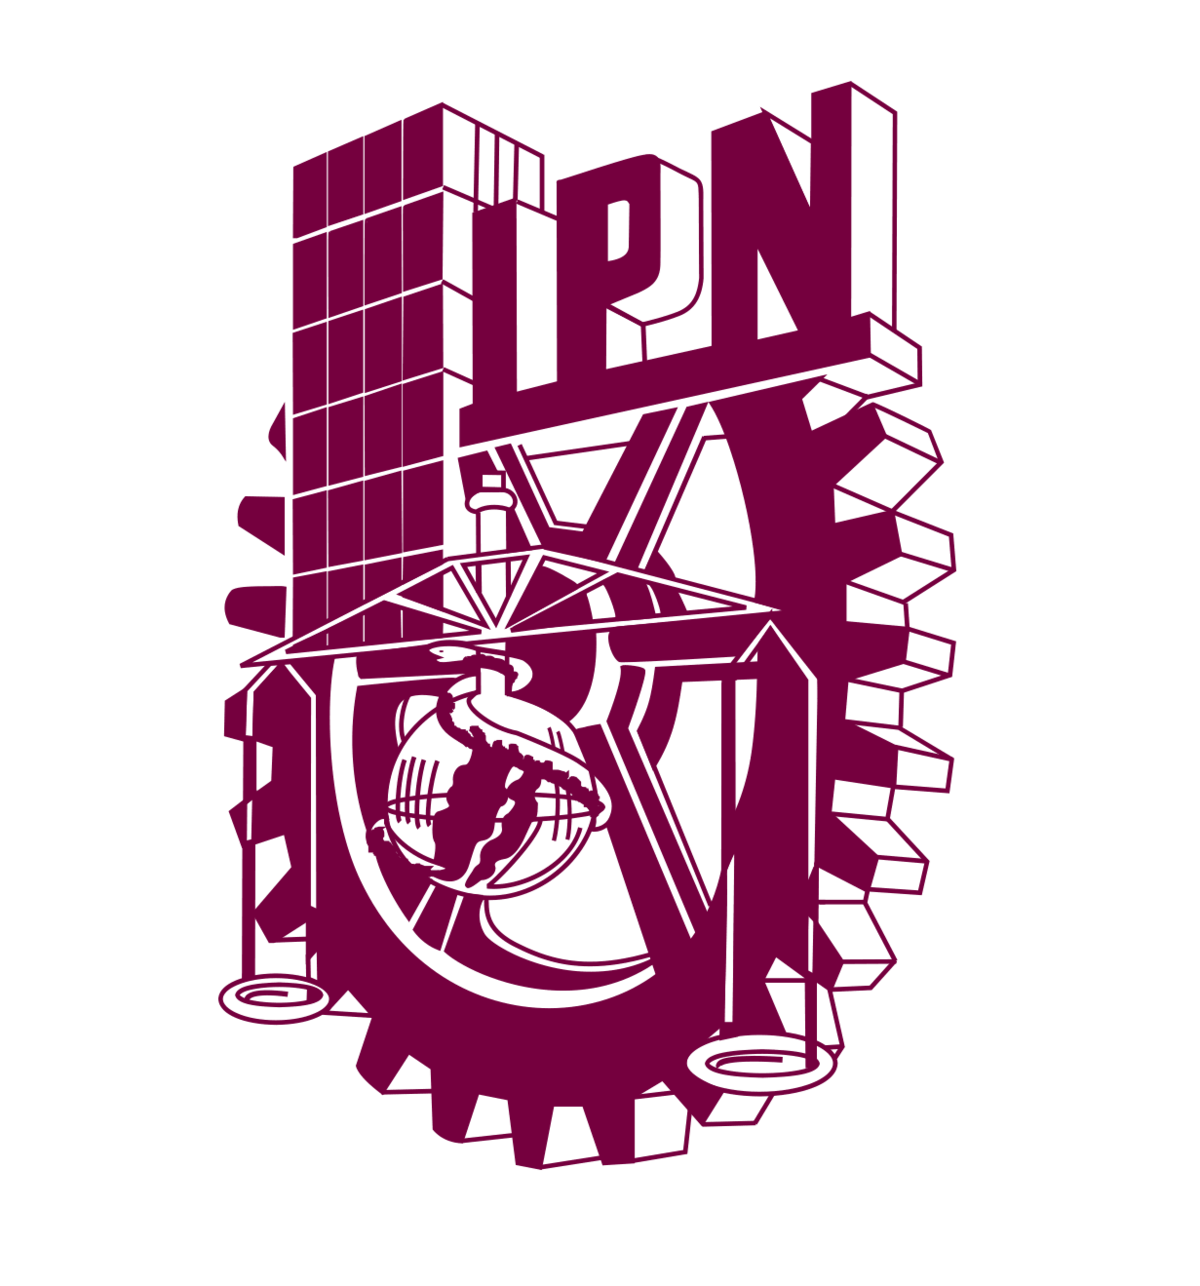
\includegraphics[width=0.22\textwidth]{Logo_IPN}}
			\hspace{0.6\textwidth}
			\subfloat{
\includegraphics[width=0.22\textwidth]{LogoEsime}}
		\end{figure}
		\centering
		{\bfseries\Huge Instituto Politécnico Nacional \par}
		\vspace{1cm}
		{\scshape\Large Ingeniería en Comunicaciones y Electrónica \par}
		\vspace{0.3cm}
		{\scshape\Large Lab. de Electricidad y Magnetismo  \par}
		\vspace{1cm}
		{\scshape\Huge ¿Toques? \par}
		\vspace{1cm}
		{\itshape\Large La Electrostática\par}
		{\Large 2CM13\par}
		\vfill
		{\Large Autores: \par}
		{\Large José Emilio Hernández Huerta \par}
		{\Large Nataly Bejarano Garduño \par}
		{\Large Daniela Elizabeth Pérez Vargas \par}
		{\Large Jesús Martinez Amac\par}
		{\Large Uriel Grimaldi Díaz  \par}
		\vfill
		{\Large Abril 2023 \par}
	\end{titlepage}
	%Indice
	 \tableofcontents
	 
	\newpage
	%Inicia el reporte
	\section{Resumen}
	La práctica consiste en la electrificación de cuerpos por medio de frotamiento ,contacto e inducción con el objetivo de observar las interacciones entre dos cuerpos, diferenciar los conductores de los aisladores y en otra instancia describir la geometría de los campos eléctricos de conductores con diferentes formas y naturalezas.
	\section{Objetivos} 
	\subsection{Generales}
	Durante la práctica, se busca observar los principios básicos de la electrostática por medio de experimentos que nos permitan aplicar los conocimientos previos en el campo y comprender cómo se pueden utilizar los principios de la electrostática en la vida cotidiana.
	\subsection{Particulares}
	Aplicar los conceptos fundamentales aprendidos de la electrostática, incluyendo los diferentes tipos de cargas eléctricas y cómo interactúan entre sí.
Identificar los diferentes procedimientos de electrificación y comprender cómo se producen las cargas eléctricas en cada uno de ellos.
Comprobar los diferentes tipos de electrificación a través de experimentos y observar los efectos de estos métodos en los objetos.
Diferenciar entre conductores y aislantes, identificar diferentes materiales que pueden actuar como conductores o aisladores.
Describir los espectros de los campos eléctricos, así como su representación en forma de espectros.
	\subsection{Introducción}
	Los humanos siempre hemos visto como la electricidad de alguna u otra forma ya sea con fenómenos meteorológicos como son los rayos o pequeñas chispas que saltan entre nuestras cobijas, inclusivamente en nuestros cuerpos desde las descargas que produce nuestro cerebro para controlar el cuerpo y las descargas de estática que experimentamos cuando nos cargamos eléctricamente. Y para poder comprender todos estos fenómenos y que es la electrostática tenemos que definir algunos conceptos importantes así como sus diferentes formulas y características. 
	\section {Marco Teórico}
	  	
	\subsection{Definición}
	Empezando con lo más simple, la electrostática es la parte de la física que estudia la electricidad en la materia y los
	fenómenos producidos por cargas eléctricas en reposo.[1]
	La electrostática describe los fenómenos que tienen lugar en sistemas donde distribuciones de carga eléctrica mantienen su localización invariante en el tiempo. En
	otras palabras, los cuerpos cargados deben permanecer en reposo. Aún más, cada porción de carga debe permanecer en reposo dentro del cuerpo cargado.[4]
	\subsection{Carga Eléctrica}
	Desde la antigua Grecia, los filósofos de la época ya conocían la existencia del ámbar y que al frotarlo este atraía trocitos de ámbar
	La carga eléctrica es una magnitud fundamental de la física, responsable de la interacción electromagnética.
	1831
	1879 Se introducen los conceptos de carga eléctrica, fuerza
	electromagnética, campo, corriente, energía potencial electrostática, etc
	James Clerk Maxwell puso las ideas de Faraday en lo que se conoce como
	las ecuaciones de Maxwell
	
	\subsection{Ley de Coulomb}
	Esta ley fue creada por Charles Coulomb (1736-1806) cuando midió las magnitudes de las fuerzas eléctricas entre objetos de carga. Cada carga puntual ejerce una fuerza sobre la otra, la cual esta dirigida a lo largo de la linea entre las cargas ($r.$) y posee igual magnitud. [2]\\
	\begin{math}
		 \vec{F} = k_{e} \frac{q_{1}q_{2}}{r{2^2}} \\  
		 k = 8.99*10^9 \frac{Nm^2}{C^2} \\
		 \epsilon_{0} = 8.55*10^-12 \frac{C^2}{Nm^2} \\
		 k = \frac{1}{4 \pi \epsilon_{0}} \\
	\end{math}
	
		\subsection{Propiedades}
		• La carga eléctrica se conserva \\
		• En un átomo neutro, las cargas 
		positiva y negativa tienen la misma
		magnitud \\
		• La carga esta cuantizada y su
		unidad fundamental es
		$e = 1.6*10^{-19}C$ \\
		• En el sistema SI la unidad de
		carga es el Coulomb \\
	\subsection{Tipos de Materiales}
	En el mundo en que vivimos los materiales tienen diferentes clasificaciones así dependiendo de sus propiedades, y en el este caso en particular hablaremos de su capacidad para conducir o transferir la carga eléctrica clasificándolos en aislantes, conductores y semiconductores 
	\subsubsection{Aislantes}
	Los electrones están ligados a los átomos por lo que la transferencias de carga es nula. Algunos ejemplos son el caucho, la madera, algunos plásticos, etc. 
	\subsubsection{Conductores}
	Los electrones son libres de moverse por el material. Ejemplos de estos son los metales, como el cobre, oro, aluminio, etc.
	\subsubsection{Semiconductores}
	Los semiconductores son un tipo especial de materiales debido a que
	presentan la característica de que se pueden comportar como conductores
	o como aislantes, dependiendo de las condiciones en que se utilicen. Por ejemplo el Silicio, Germanio, Azufre, Indio, etc. 

	\section{Descripción de materiales}
Péndulo\\
Sistema en equilibrio a partir de una base de metal, un hilo y una esfera de sauco
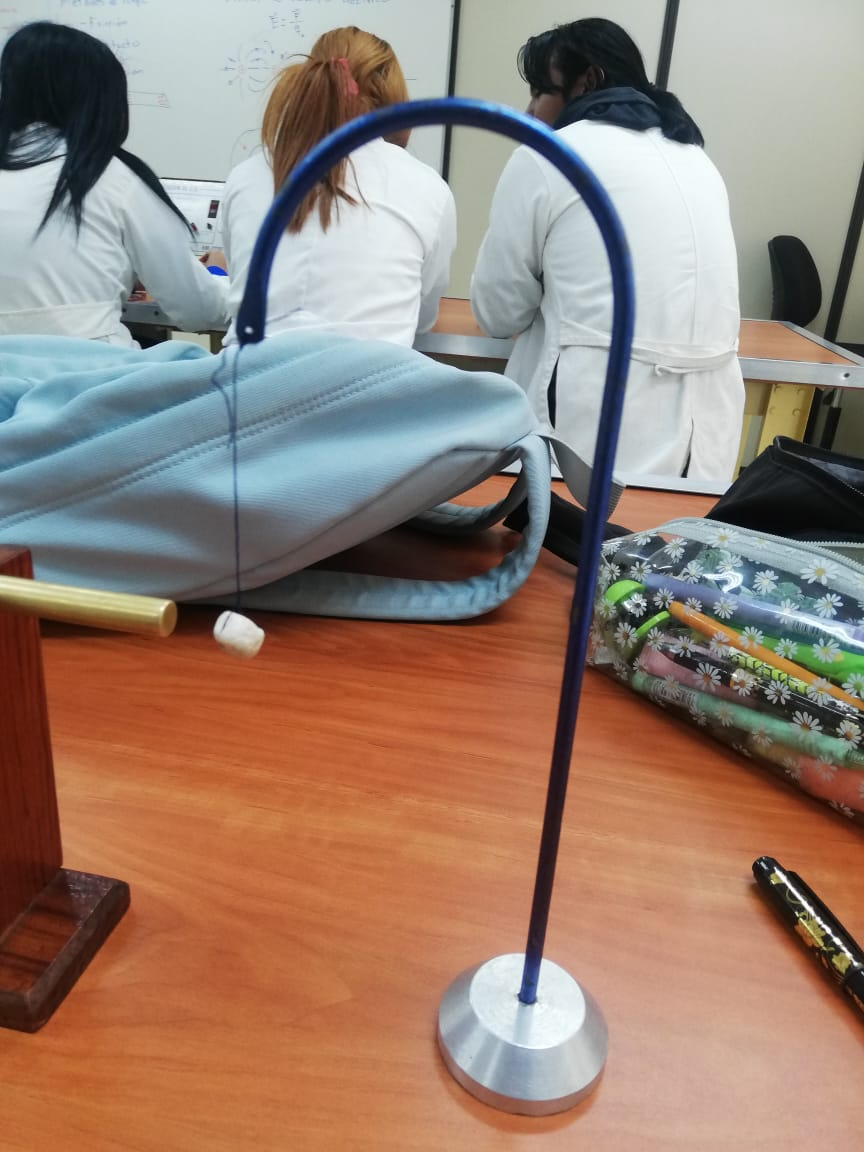
\includegraphics[width=0.1\textwidth]{Pendulo}

Cables\\ 
Son cables de cobre con un aislante de plástico color rojo para conectar la cuba con el demás sistema 
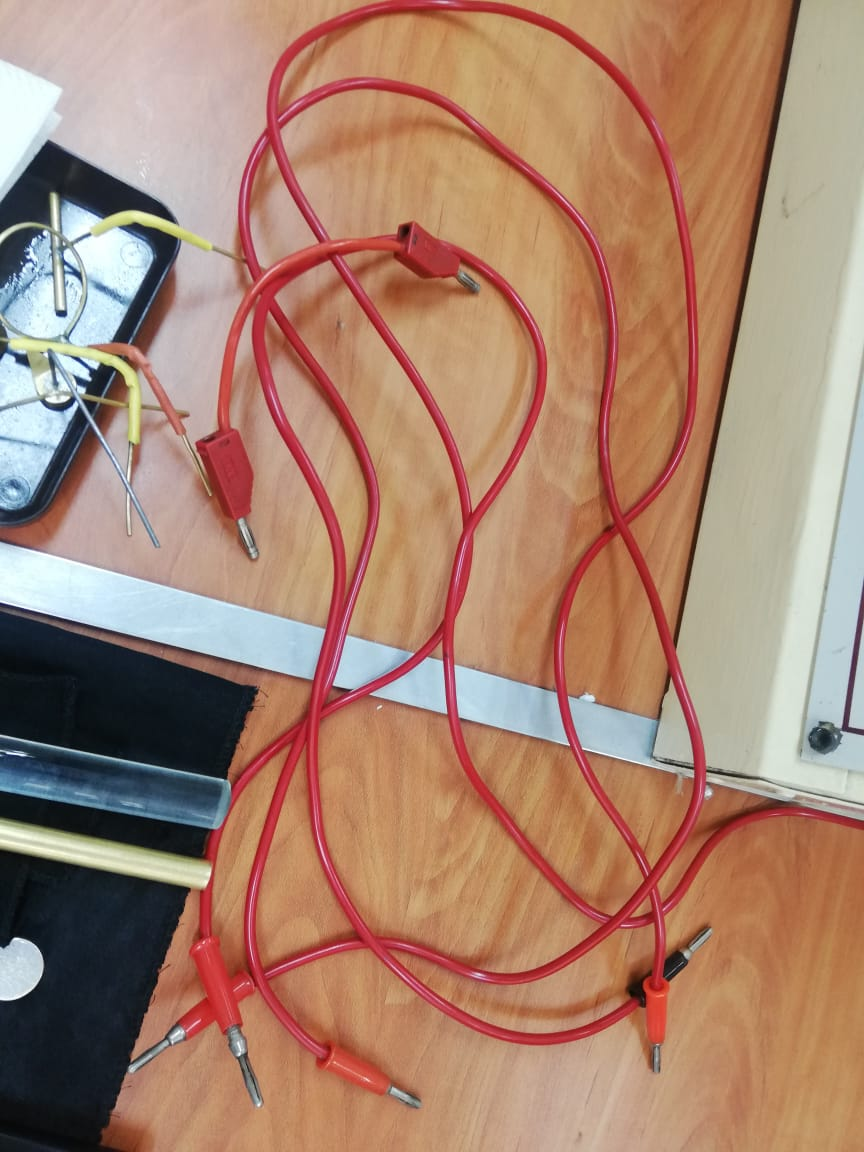
\includegraphics[width=0.1\textwidth]{Cables}

Soporte \\
Es un soporte de madera que sirve pasa colocar las barras de vidrio y de poliestireno 
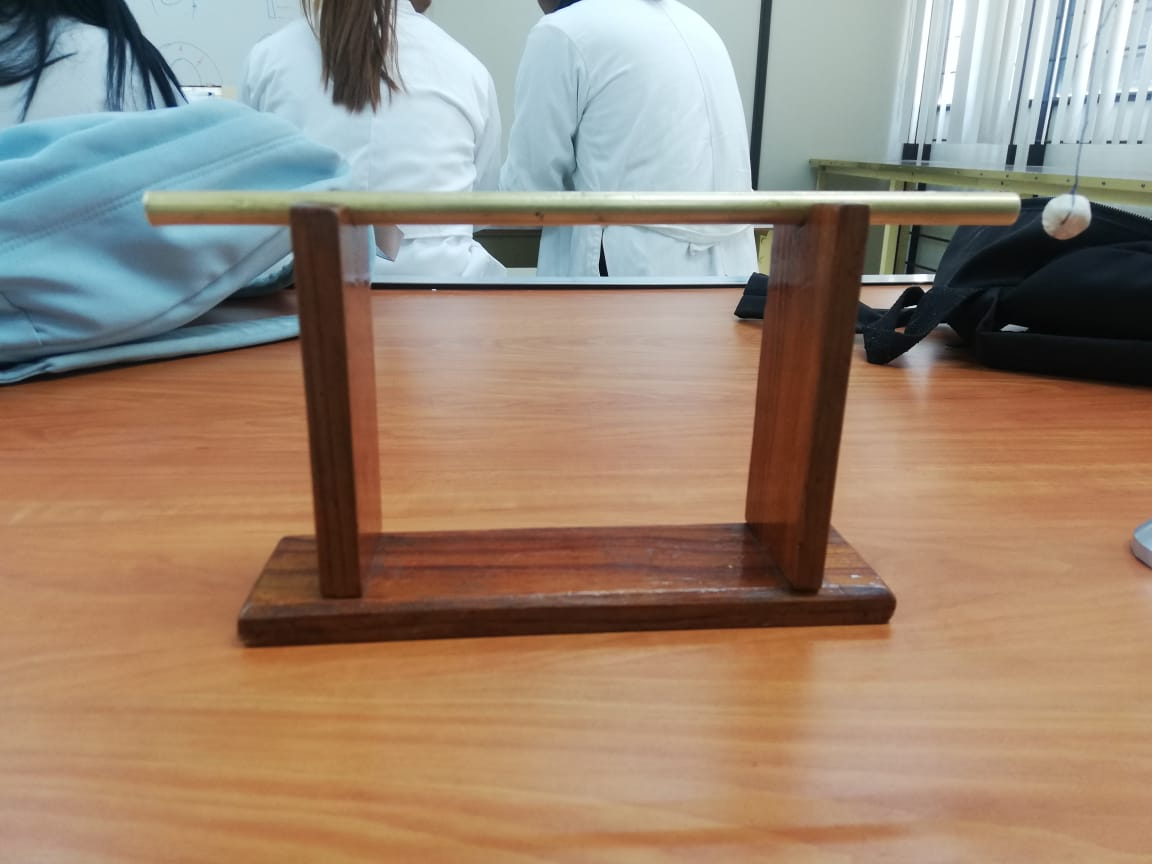
\includegraphics[width=0.1\textwidth]{Soporte}

Barra de metal \\
Es una barra de metal larga excelente conductor 
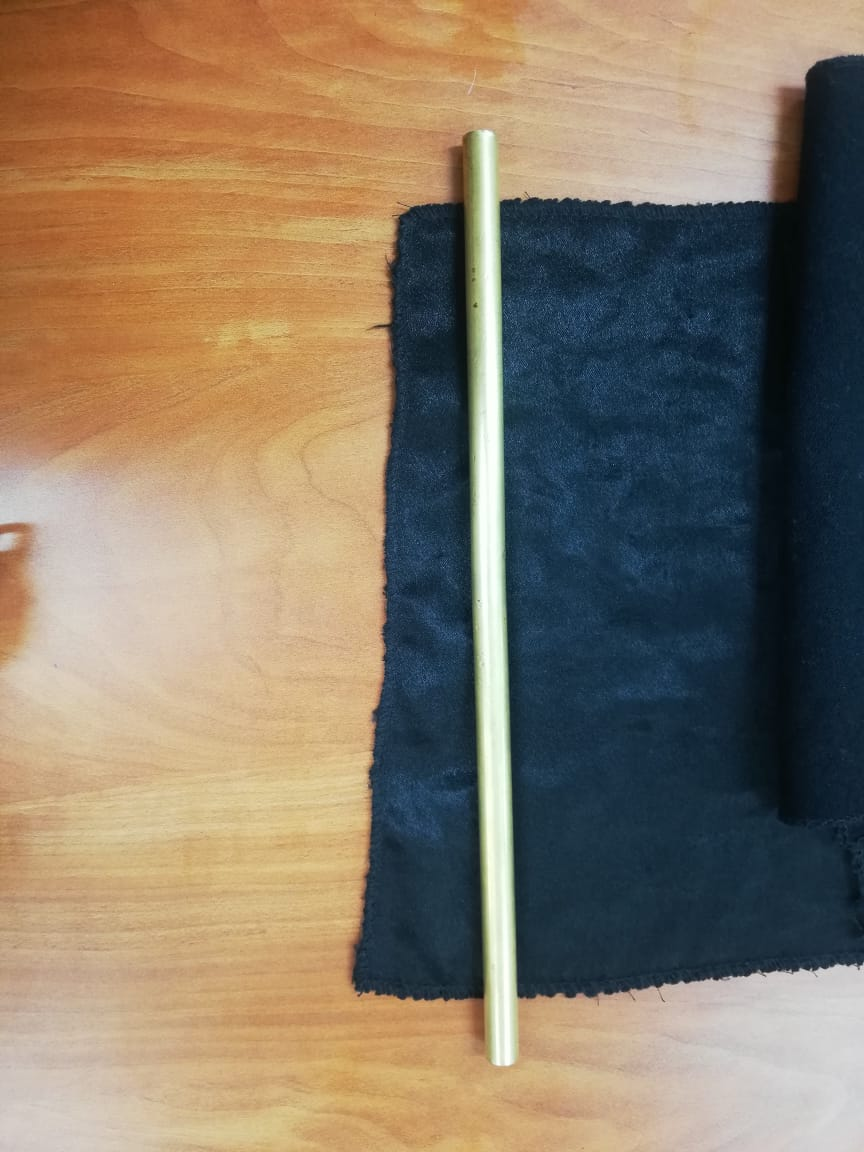
\includegraphics[width=0.1\textwidth]{Barra de metal}

Jumper \\
Sirve para conectar dos cosas a la misma vez, o pasar corriente 
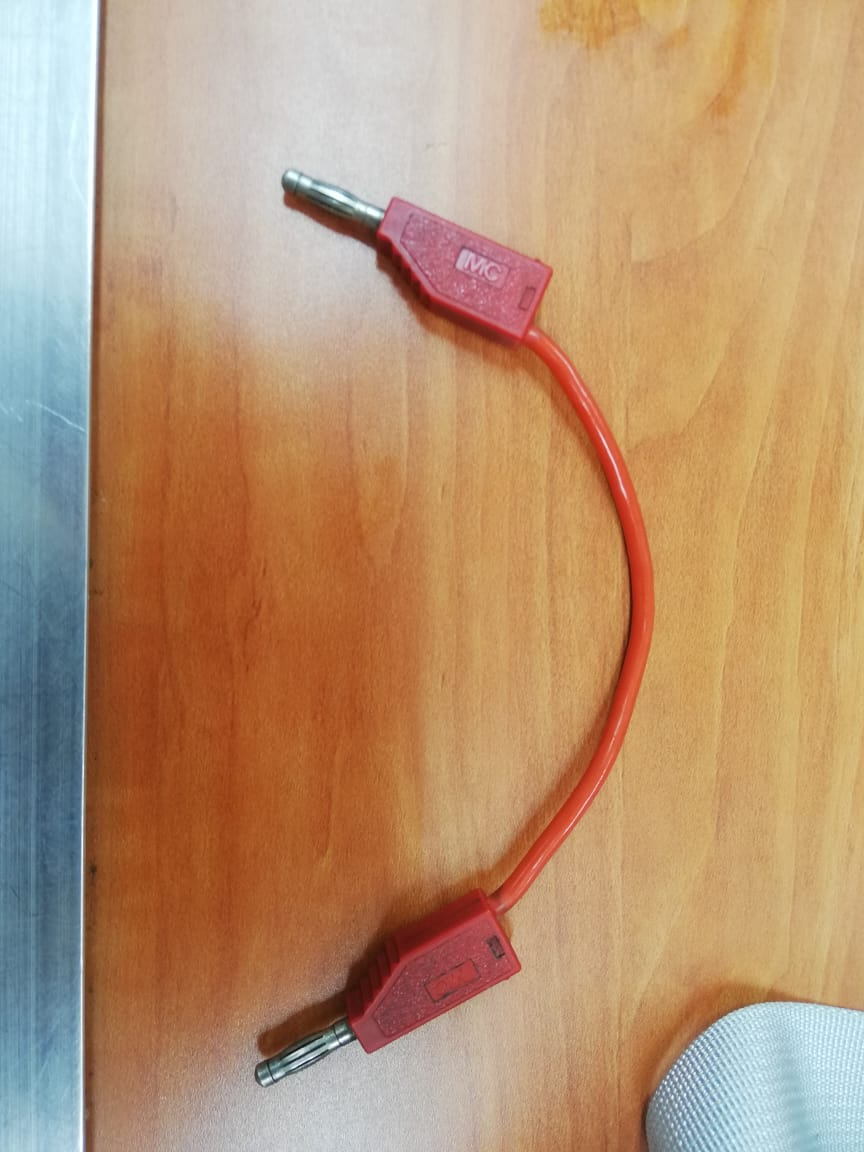
\includegraphics[width=0.1\textwidth]{Jumper}

Barra de poliestireno \\
Es una barra grande de poliestireno con una forma cilíndrica 
\includegraphics[width=0.1\textwidth]{Barra de poliestireno}

Electrodos \\
Estos son los que están conectados al generador y a la cuba para ver el efecto del aserrín con las cargas  
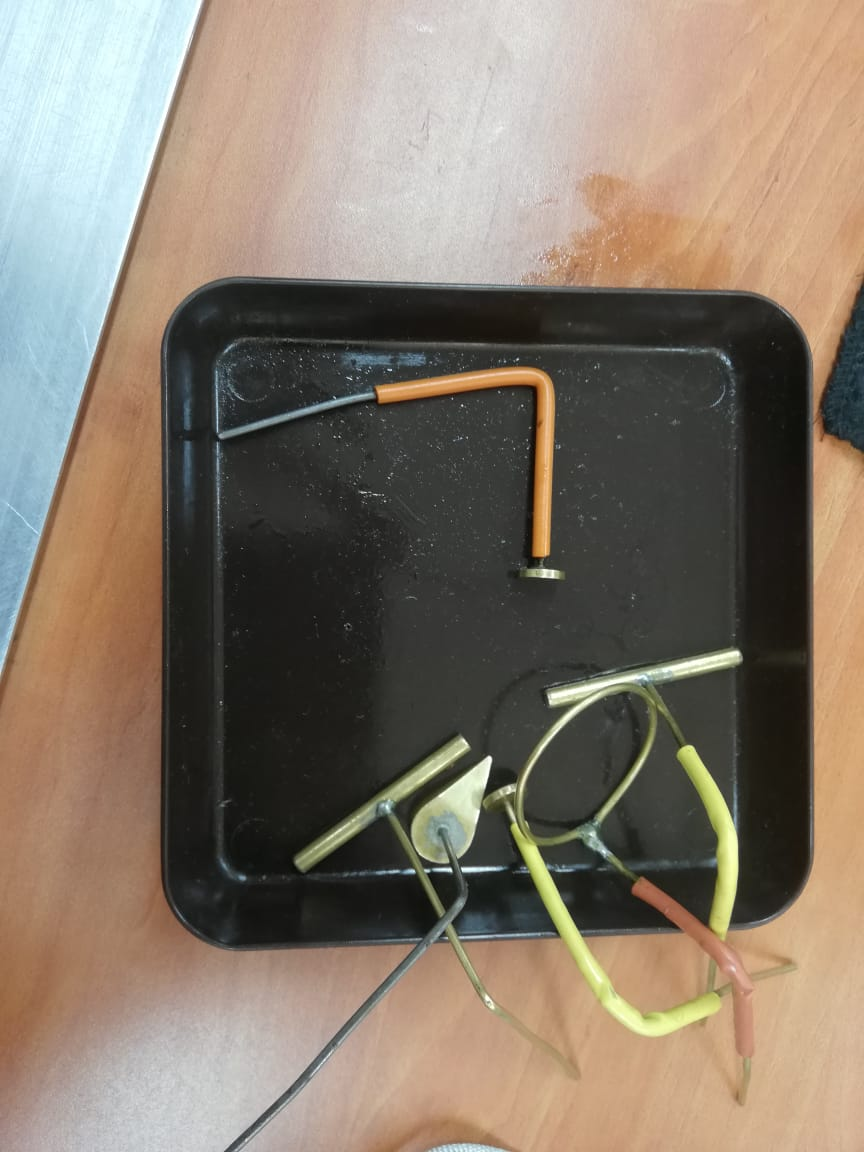
\includegraphics[width=0.1\textwidth]{Electrodos}

Cuba \\
Es el recipiente en donde se vierte el aceite y el aserrín  
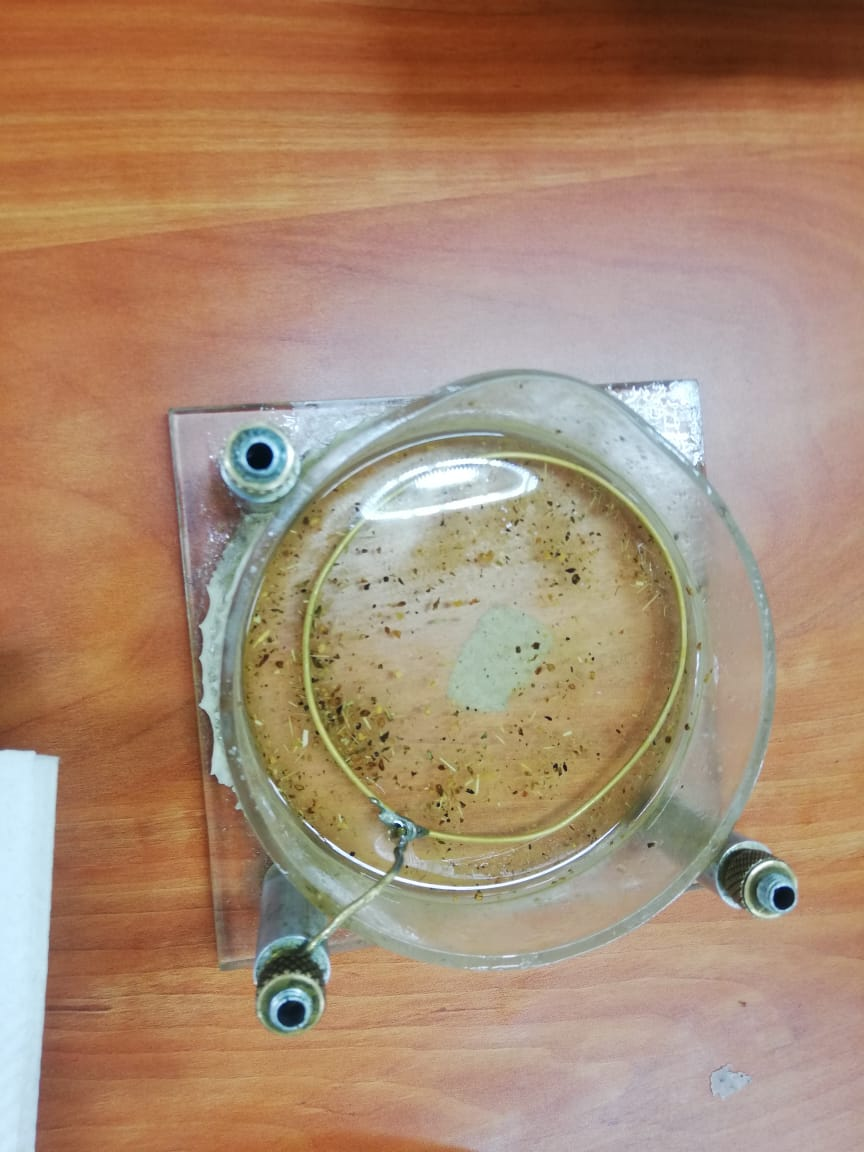
\includegraphics[width=0.1\textwidth]{Cuba}

Barra de vidrio \\
Es una barra grande de fibra de vidrio con la que trabajamos más 
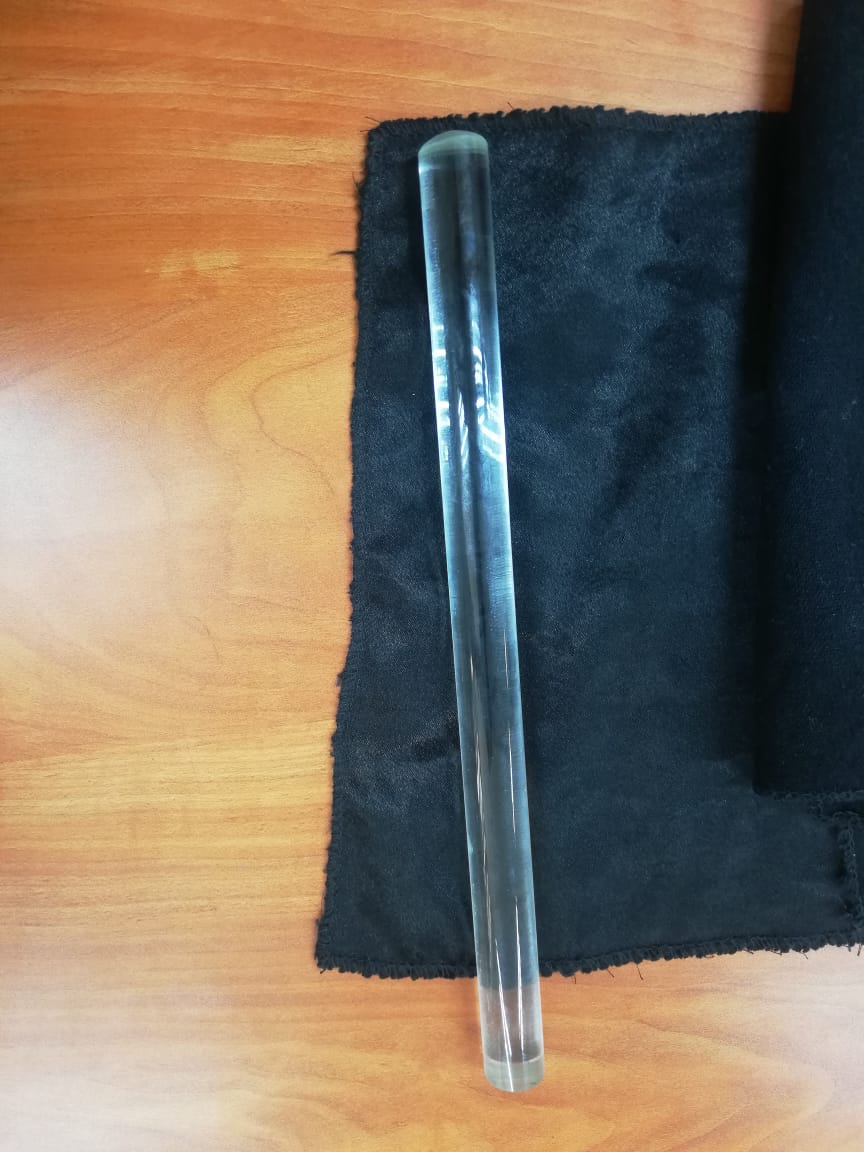
\includegraphics[width=0.1\textwidth]{Barra de vidrio}

	\section{Desarrollo Experimental}
	Experimento 1 Electrización de un cuerpo
	Existen tres procedimientos por el medio de los cuales los cuerpos pueden electrizarse: por frotamiento, por contacto y/o por inducción. 

	Experimento 1.1 Electrización por frotamiento 
	(este experimento lo dividimos en tres etapas) 
	\begin{enumerate}
		\item Como primer paso, frotamos la barra de vidrio con el paño de lana y la acercamos a algunos trazos de papel, para posteriormente ver su reacción 
		\item Nuestro segundo paso fue, frotar la barra de vidrio con el paño de lana y lo acercamos (sin tocar) a la esfera de sauco del péndulo 
		\item Por último, frotamos la barra de poliestireno y la aproximamos al péndulo eléctrico, (sin tocar la esfera de sauco)
	\end{enumerate}
	Experimento 1.2 Electrización por contacto. 
(este experimento se divide en dos fases) 
\begin{enumerate}
	\item Como primera fase, tomamos la barra de vidrio (cargada previamente) por frotamiento del paño de lana, y la pusimos en contacto con el electrodo de prueba plano, así mismo lo acercamos a la esfera del péndulo eléctrico. 
	\item Antes de comenzar la segunda fase, descargamos el electrodo de prueba con los dedos, y posteriormente tomamos la barra de poliestireno (cargada previamente) por frotamiento del paño de lana, y la pusimos en contacto con el electrodo de prueba plano, así mismo lo acercamos a la esfera del péndulo eléctrico.  
\end{enumerate}
Experimento 1.3 Electrización por inducción. 
(este experimento se divide en dos partes) 
\begin{enumerate}
	\item Primero, frotamos la barra de vidrio con el paño de lana y la acercamos a la barra de metal (sin tocarla), para posteriormente observar la esfera del péndulo eléctrico, y sin dejar de observar alejamos la barra de vidrio cargada.
	\item Después, repetimos el experimento anterior, solo que antes de retirar la barra de vidrio cargada eléctricamente, tocamos con el dedo la barra de metal. 
\end{enumerate}
II Clases de Carga Eléctrica y Fuerzas de Origen Eléctrico.
Procedimiento. Experimento II.I
(se divide en dos fases)
\begin{enumerate}
	\item Colocamos la barra de poliestireno en el soporte aislante frente al péndulo, y cargamos la barra de vidrio por frotamiento con el paño de lana, para posteriormente observar que pasa con el péndulo. 
	\item Después descargamos la barra de vidrio y la colocamos en el soporte aislante, en lugar de la barra de poliestireno, para cargar esta última con el paño de lana y repetir el experimento   
\end{enumerate}
IV. Espectros de Campo Eléctrico. 
IV.I Armamos el dispositivo como lo indicaba el practicarío, para después poner a funcionar el generador y observar lo que sucede con el aserrín 
IV.II Posteriormente desconectamos el generador y descargamos la esfera tocándola con el alambre, para conectar la tierra y mover el aserrín de posición para generar la nueva reacción, previamente invirtiendo las conexiones en los portaelectrodos, de la manera en que la lenteja estuviera conectada a la esfera del generador. 
IV.III Después cambiamos los electrodos (lenteja y arillo), por otro par, de modo que se observara un campo formado por: 
\begin{enumerate}
	\item Dos cargas puntuales de diferente signo 
	\item Dos cargas puntuales del mismo signo 
	\item Dos placas paralelas cargadas de diferente signo que simulen un condensador de placas paralelas 
	\item Dos arillos circulares cargados con diferente carga, de tal manera que simulen un condensador de placas cilíndricas 
	\item Un cuerpo con punta y una placa cargada con signo contrario 
\end{enumerate}
\section{Análisis y resultados}
\subsection*{1.1.- Electrización por frotamiento}
\subsubsection*{Procedimiento 1}
Se utilizo la barra de vidrio y el paño de lana, como primer paso frotamos la barra de vidrio con el paño de lana para generar fricción en la barra de vidrio, esto genera un campo eléctrico, posterior mente se colocaron pequeños trozos de papel, como siguiente paso se acerca la barra de vidrio a los pequeños trozos de papel.

\begin{figure}[h]
\centering
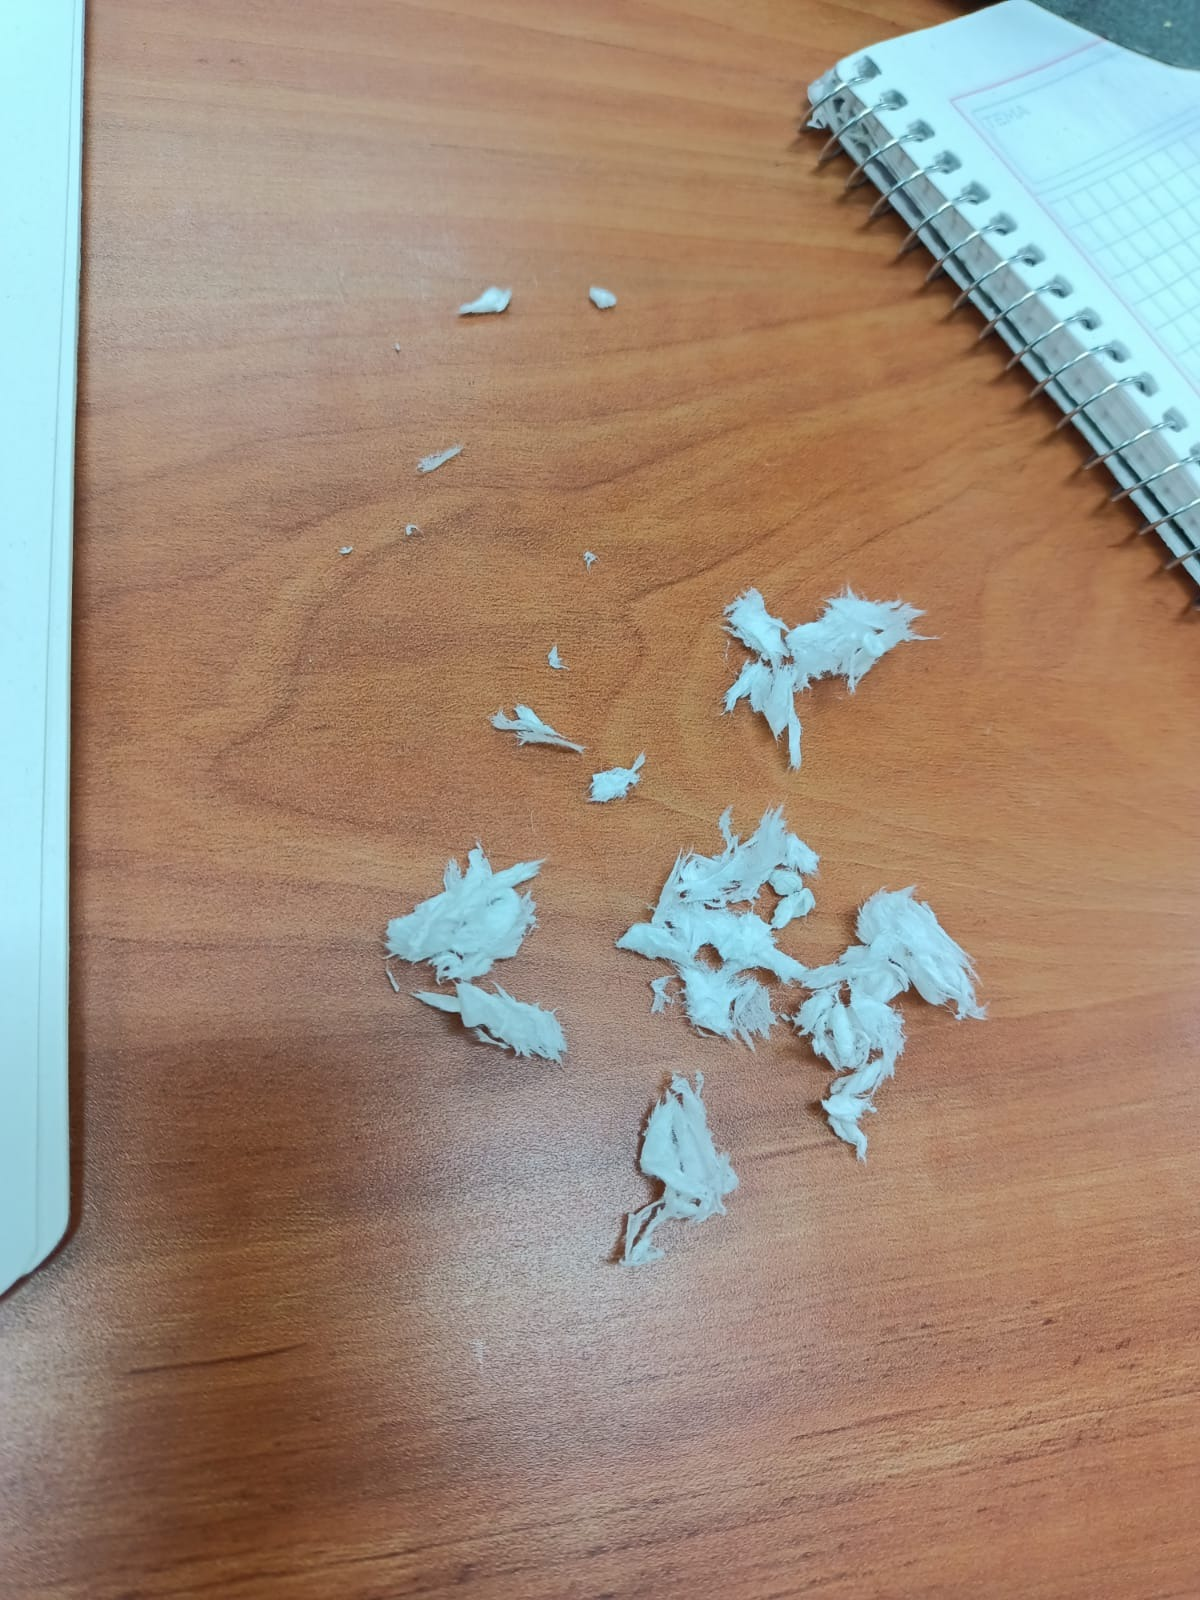
\includegraphics[scale=0.07]{P2}
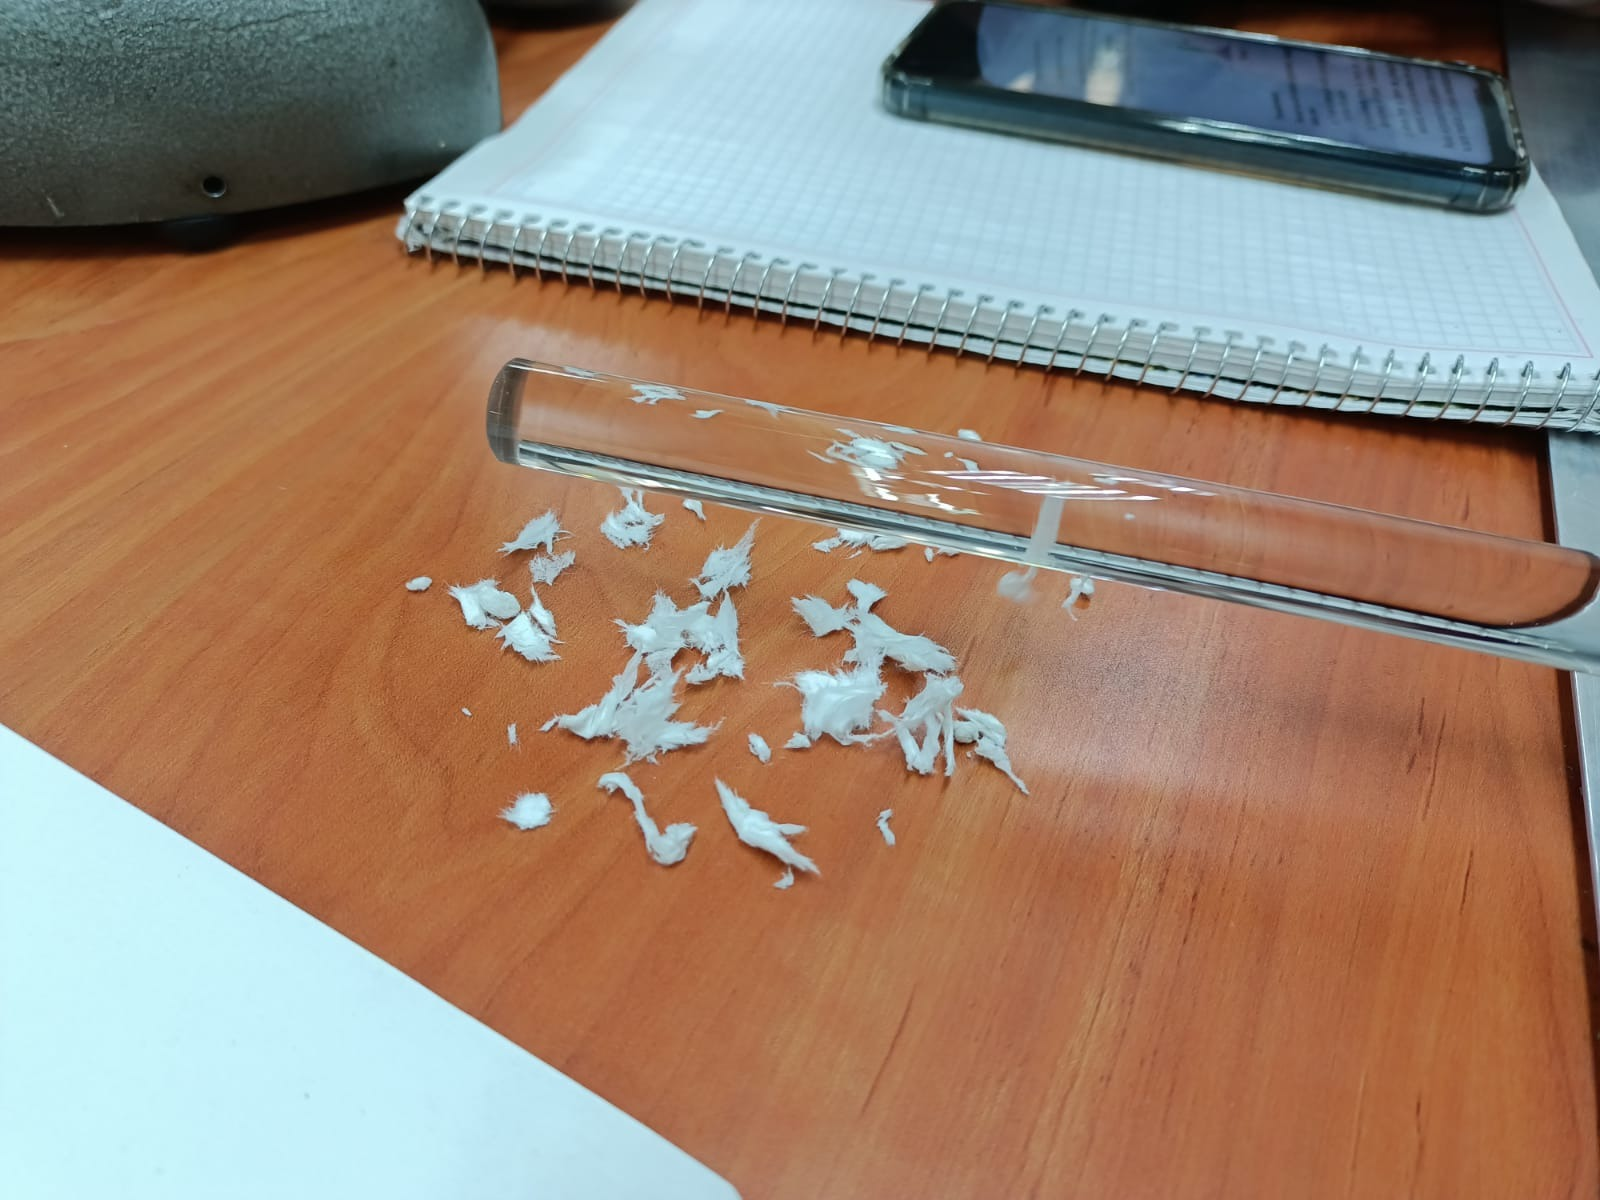
\includegraphics[scale=0.09]{P1}
\caption{Resultado}
\end{figure}

Como resultado observamos que al frotar el paño de lana en la barra de vidrio genero un campo eléctrico, que al momento de acercar la barra de vidrio provoco una fuerza de atracción provocando que los tozos de papel sean atraídos por la barra de vidrio.

\subsubsection*{Procedimiento 2}

Se utilizo la barra de vidrio y el paño de lana, como primer paso nuevamente frotamos la barra de vidrio con el paño de lana, para generar fricción en la barra de vidrio, esto genera un campo eléctrico, como siguiente paso aproximamos la barra de vidrio a la esfera de sauco del péndulo eléctrico.

\begin{figure}[h]
\centering
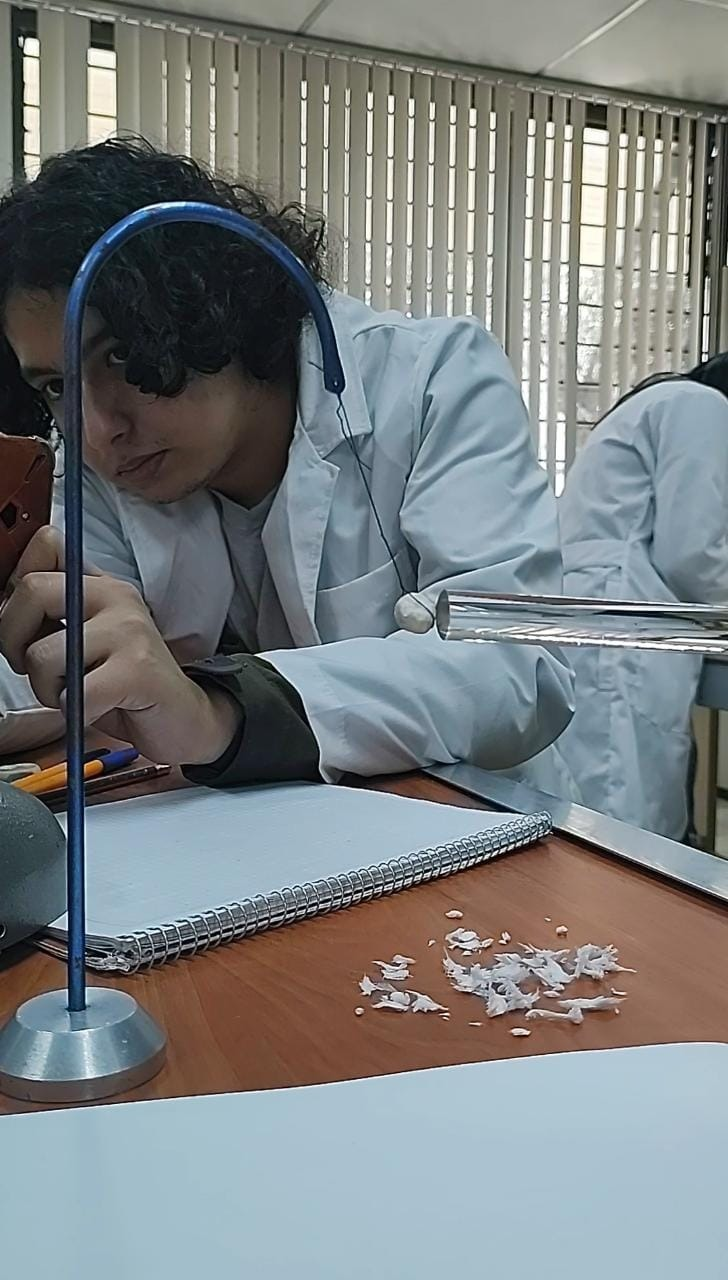
\includegraphics[scale=0.07]{P3}
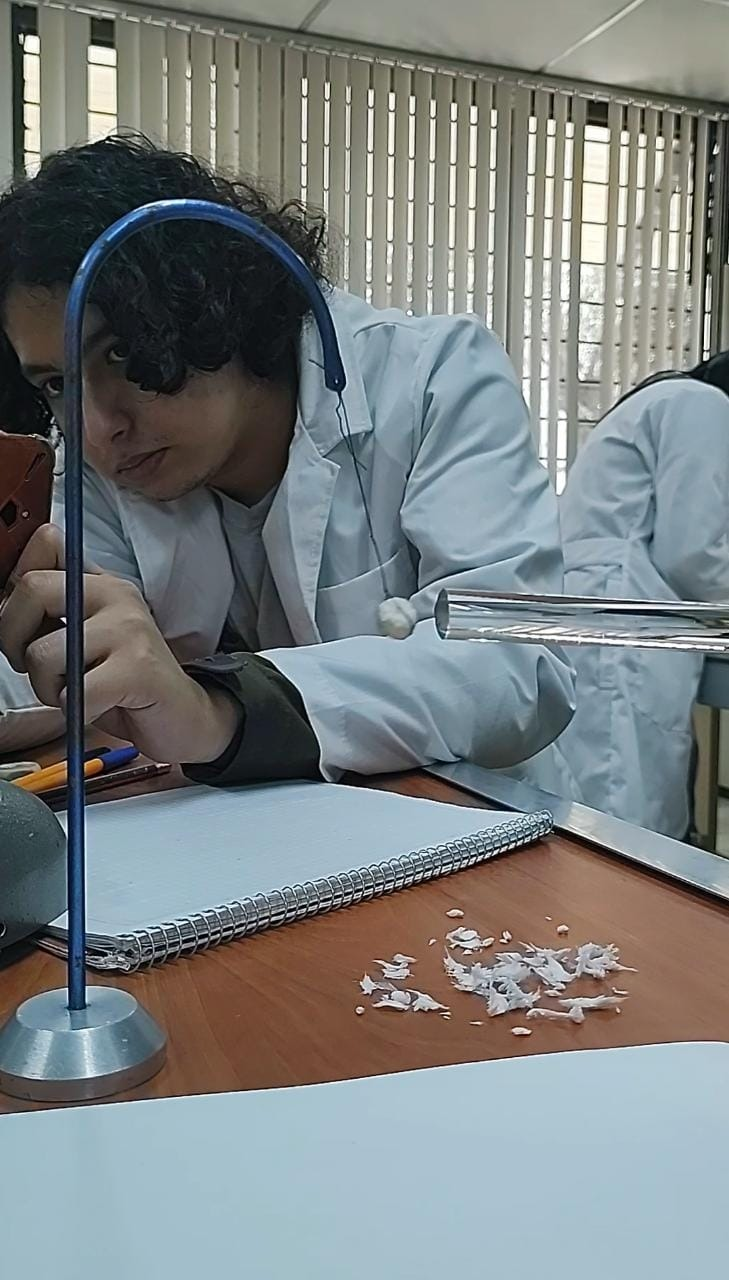
\includegraphics[scale=0.07]{P4}
\caption{Resultado}
\end{figure}

Como resultado observamos que al frotar nuevamente el paño de lana en la barra de vidrio genere un campo eléctrico, que al momento de acercar la barra de vidrio a la esfera de sauco del péndulo eléctrico provoco una fuerza de atracción provocando que la esfera de sauco sea atraída por la barra de vidrio.
\subsubsection*{Procedimiento 3}
Se utilizo la barra de poliestireno y el paño de lana, como primer paso nueva mente frotamos la barra de poliestireno con el paño de lana para generar fricción en la barra de poliestireno, esto genera un campo eléctrico, como siguiente paso aproximamos la barra de poliestireno a la esfera de sauco del péndulo eléctrico.

\begin{figure}[h]
\centering
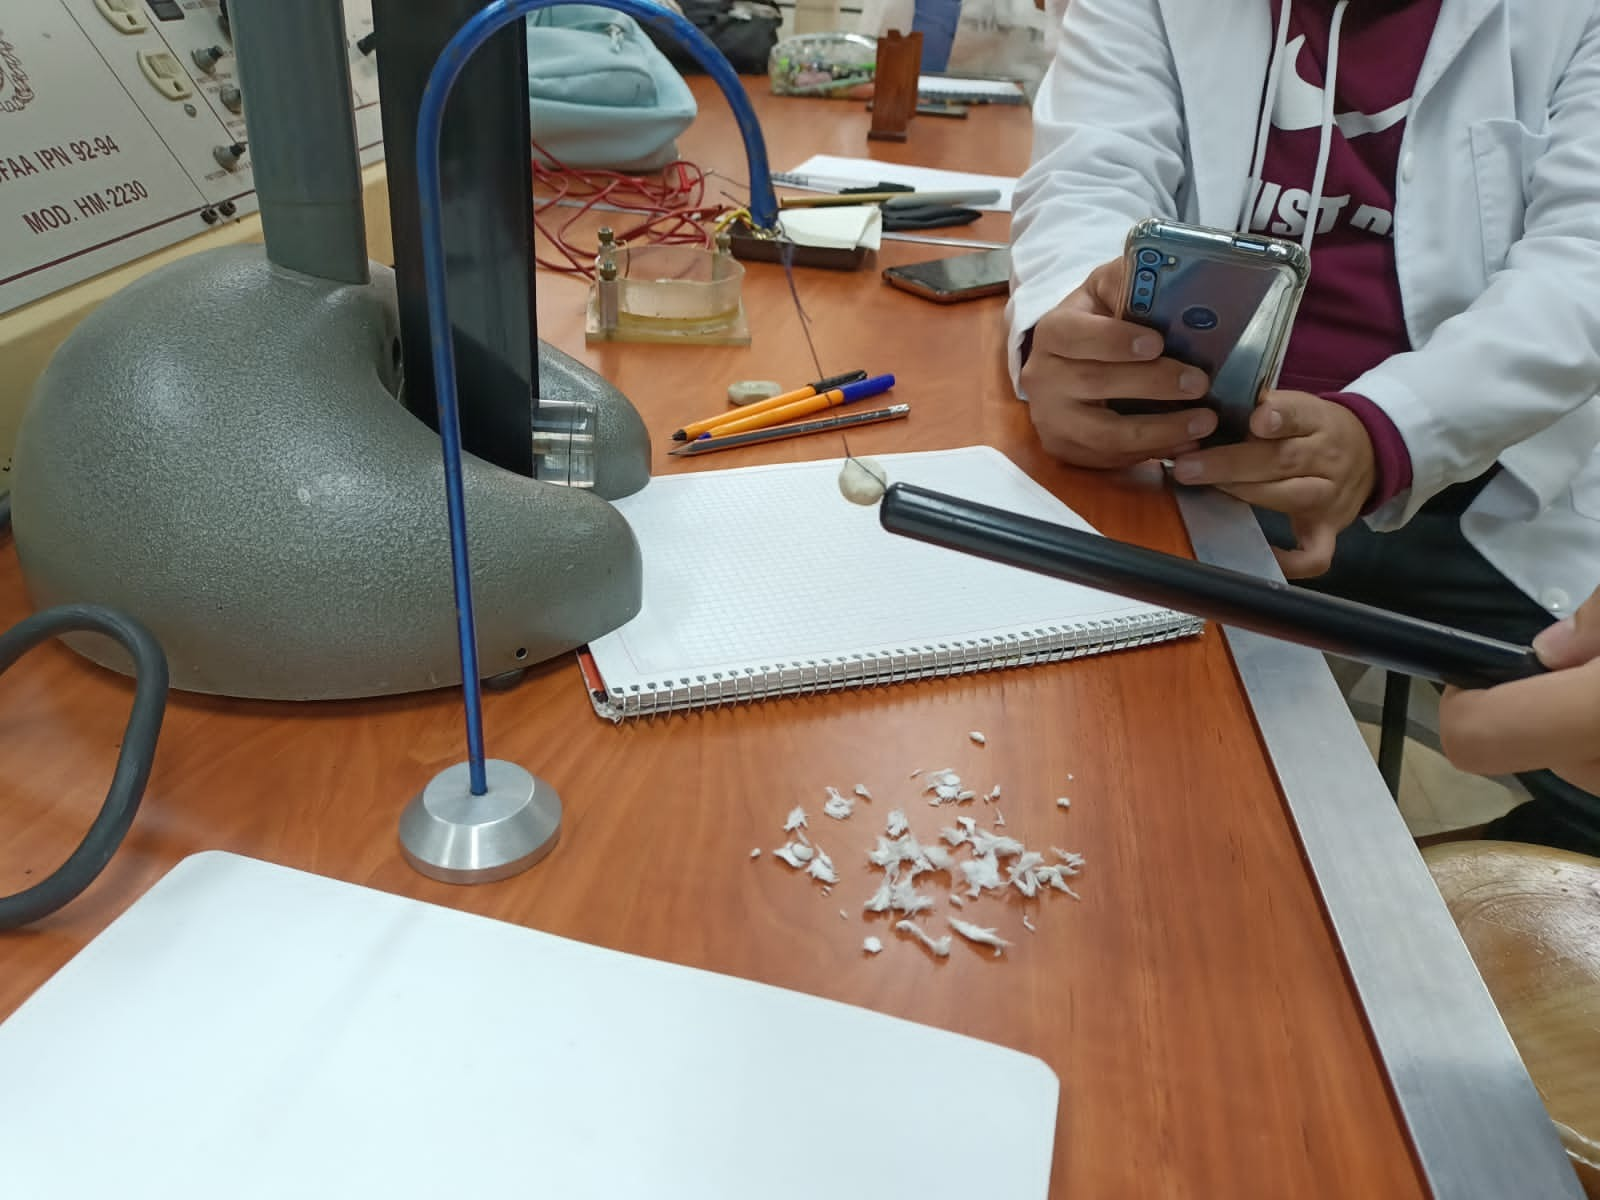
\includegraphics[scale=0.07]{P5}
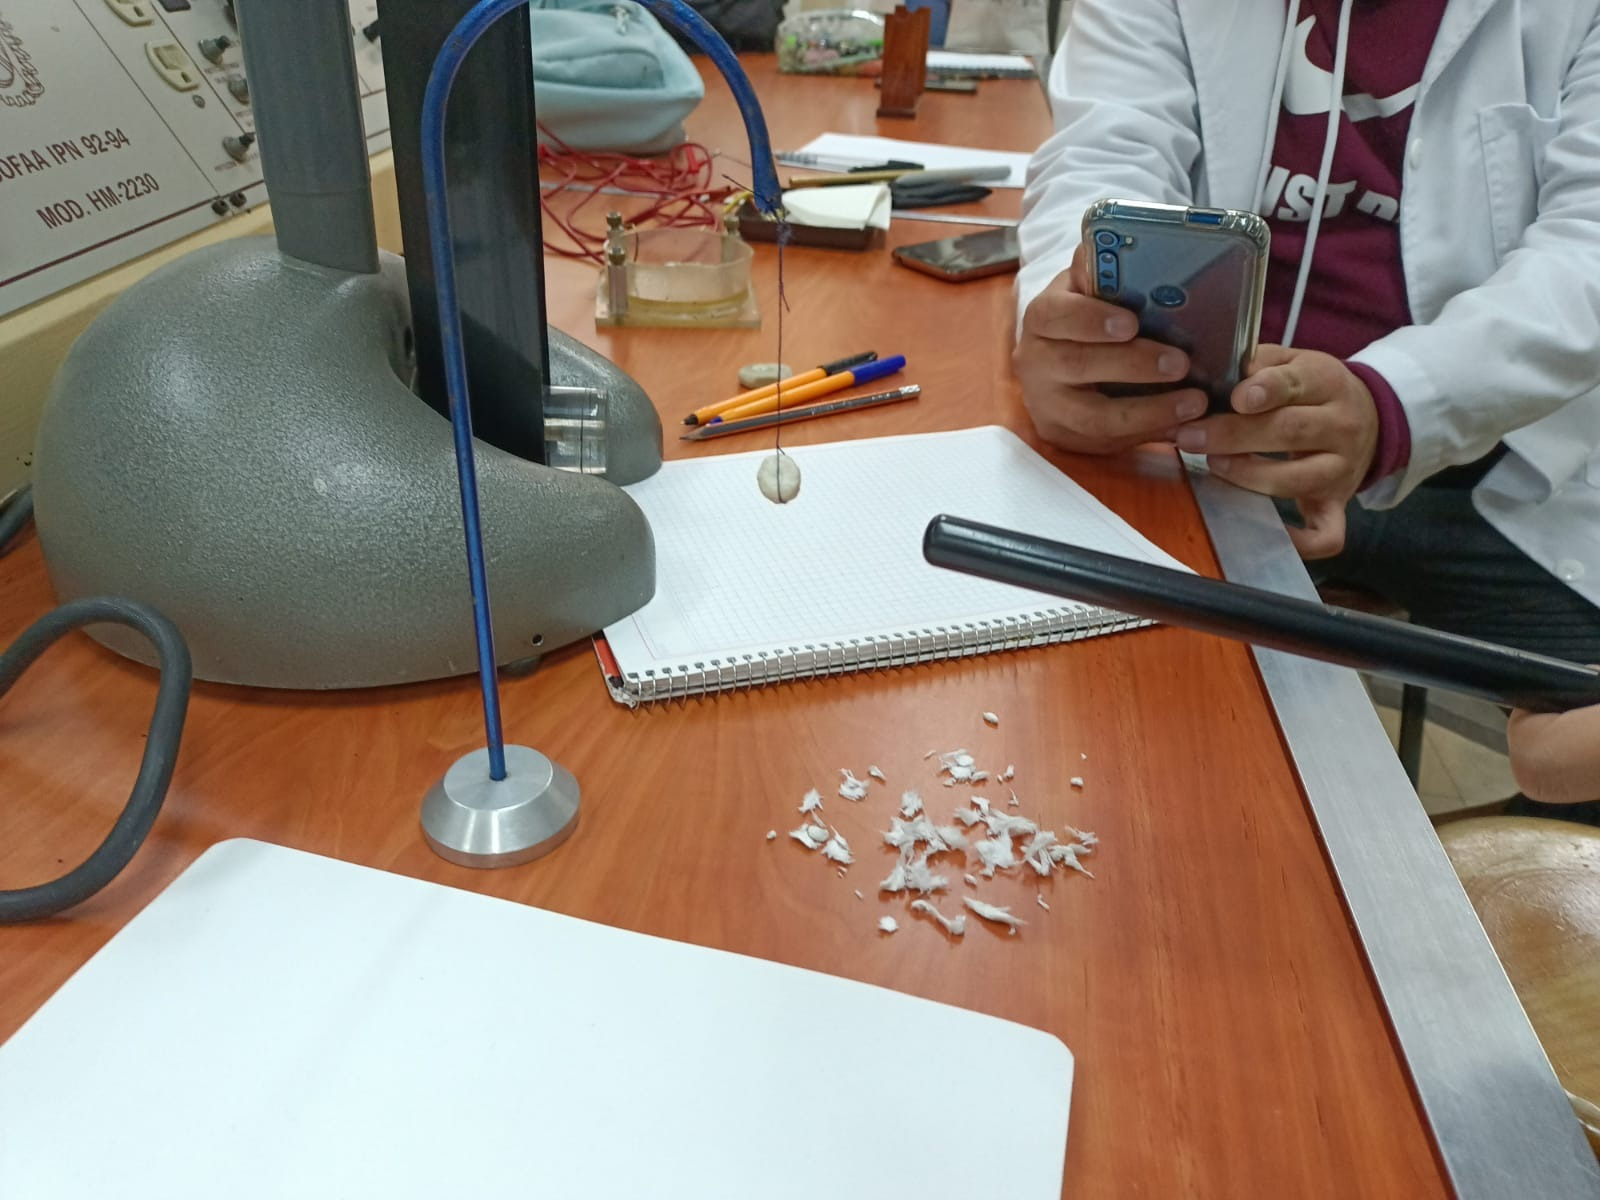
\includegraphics[scale=0.07]{P6}
\caption{Resultado}
\end{figure}

Como resultado observamos que al frotar nuevamente el paño de lana en la barra de poliestireno genere un campo eléctrico, que al momento de acercar la barra de poliestireno a la esfera de sauco del péndulo eléctrico provoco una fuerza de atracción provocando que la esfera de sauco sea atraída por la barra de poliestireno.

\subsection*{1.2.- Electrización por contacto}
\subsubsection*{Procedimiento 1}
Se utilizo la barra de vidrio, cargada previamente por el frotamiento del paño de lana a si generando un campo eléctrico, como siguiente paso pusimos en contacto con el electrodo de prueba plano, el siguiente paso fue acercarlo a la esfera del péndulo eléctrico.

\begin{figure}[h]
\centering
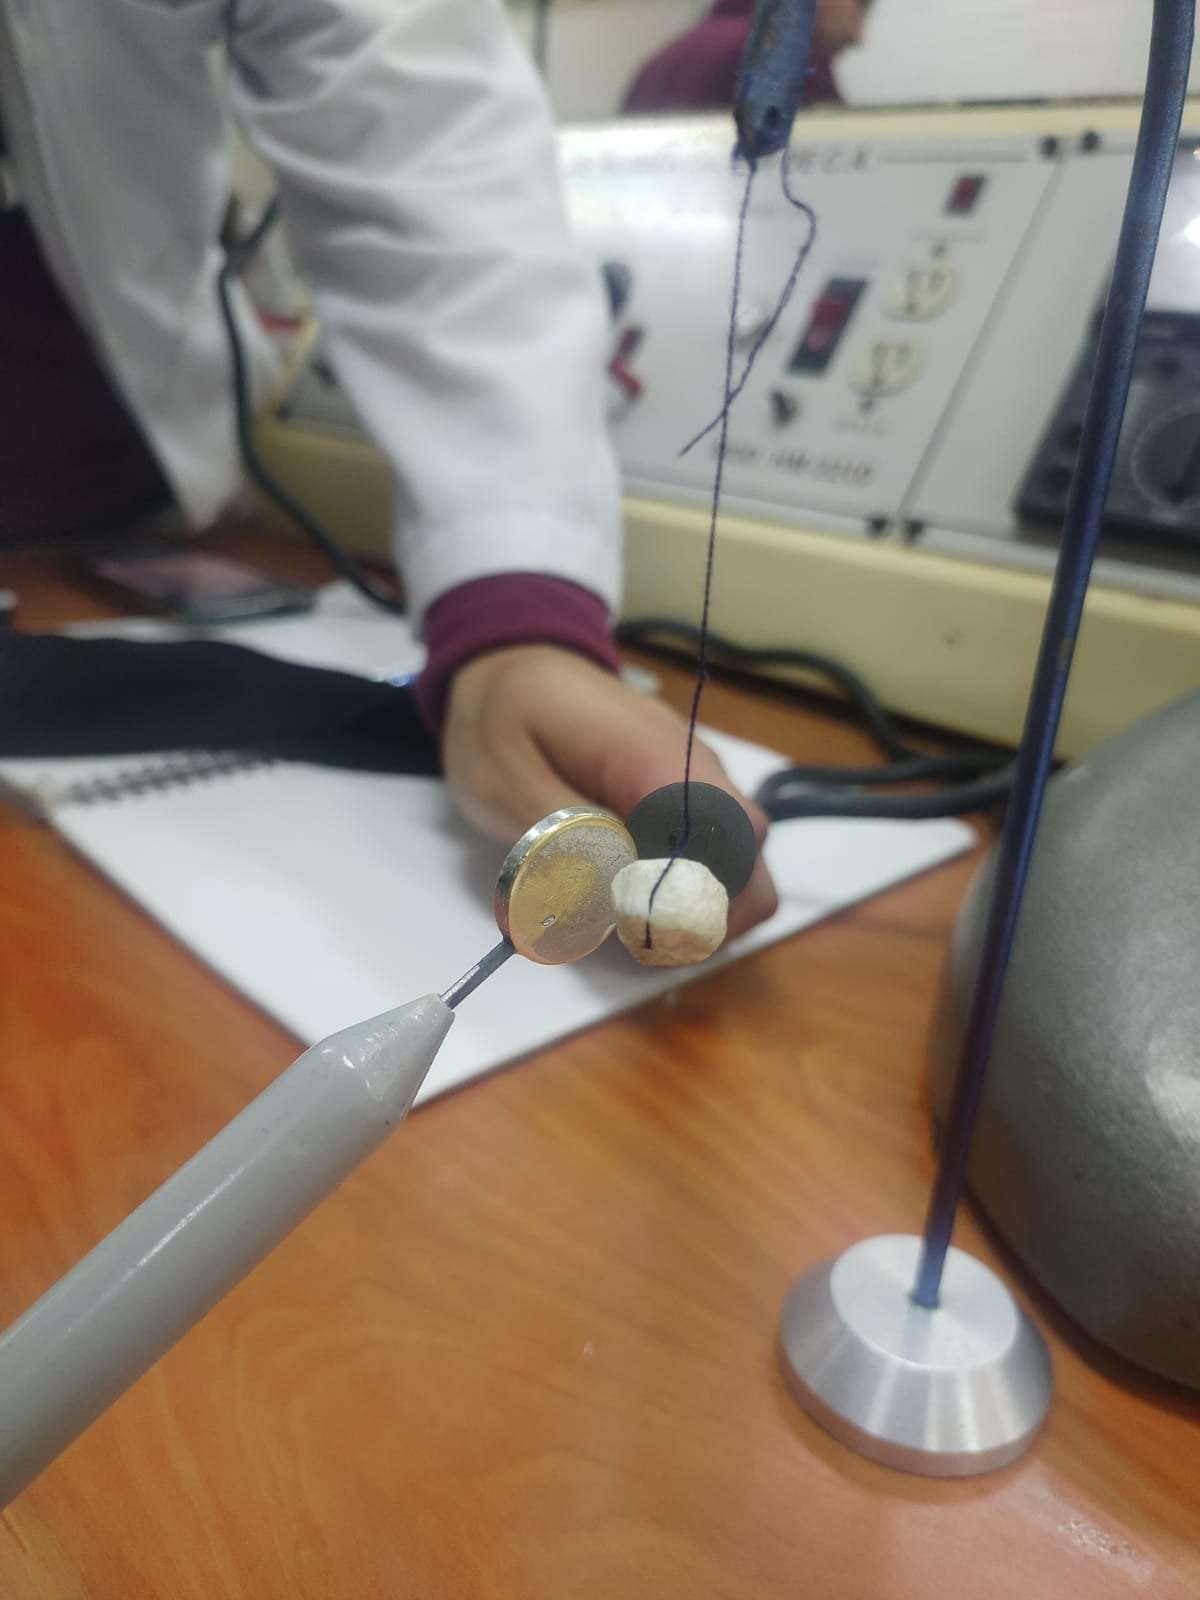
\includegraphics[scale=0.07]{P7}
\caption{Resultado}
\end{figure}

Como resultado observamos que al frotar el paño de lana con la barra de vidrio, genera un campo eléctrico y al unirlo al electrodo de prueba plano la carga de la barra de vidrio se pasa al electrodo de prueba de plano, así generando una fuerza de atracción provocando que la esfera de sauco sea atraída por la barra de vidrio y el electrodo de prueba plano.
\subsubsection*{Procedimiento 2}
Se utilizo la barra de poliestireno, cargada previamente por el frotamiento del paño de lana a si generando un campo eléctrico, como siguiente paso pusimos en contacto con el electrodo de prueba plano descargado previamente con la llama de los dedos, el siguiente paso fue acercarlo a la esfera del péndulo eléctrico.

\begin{figure}[h]
\centering
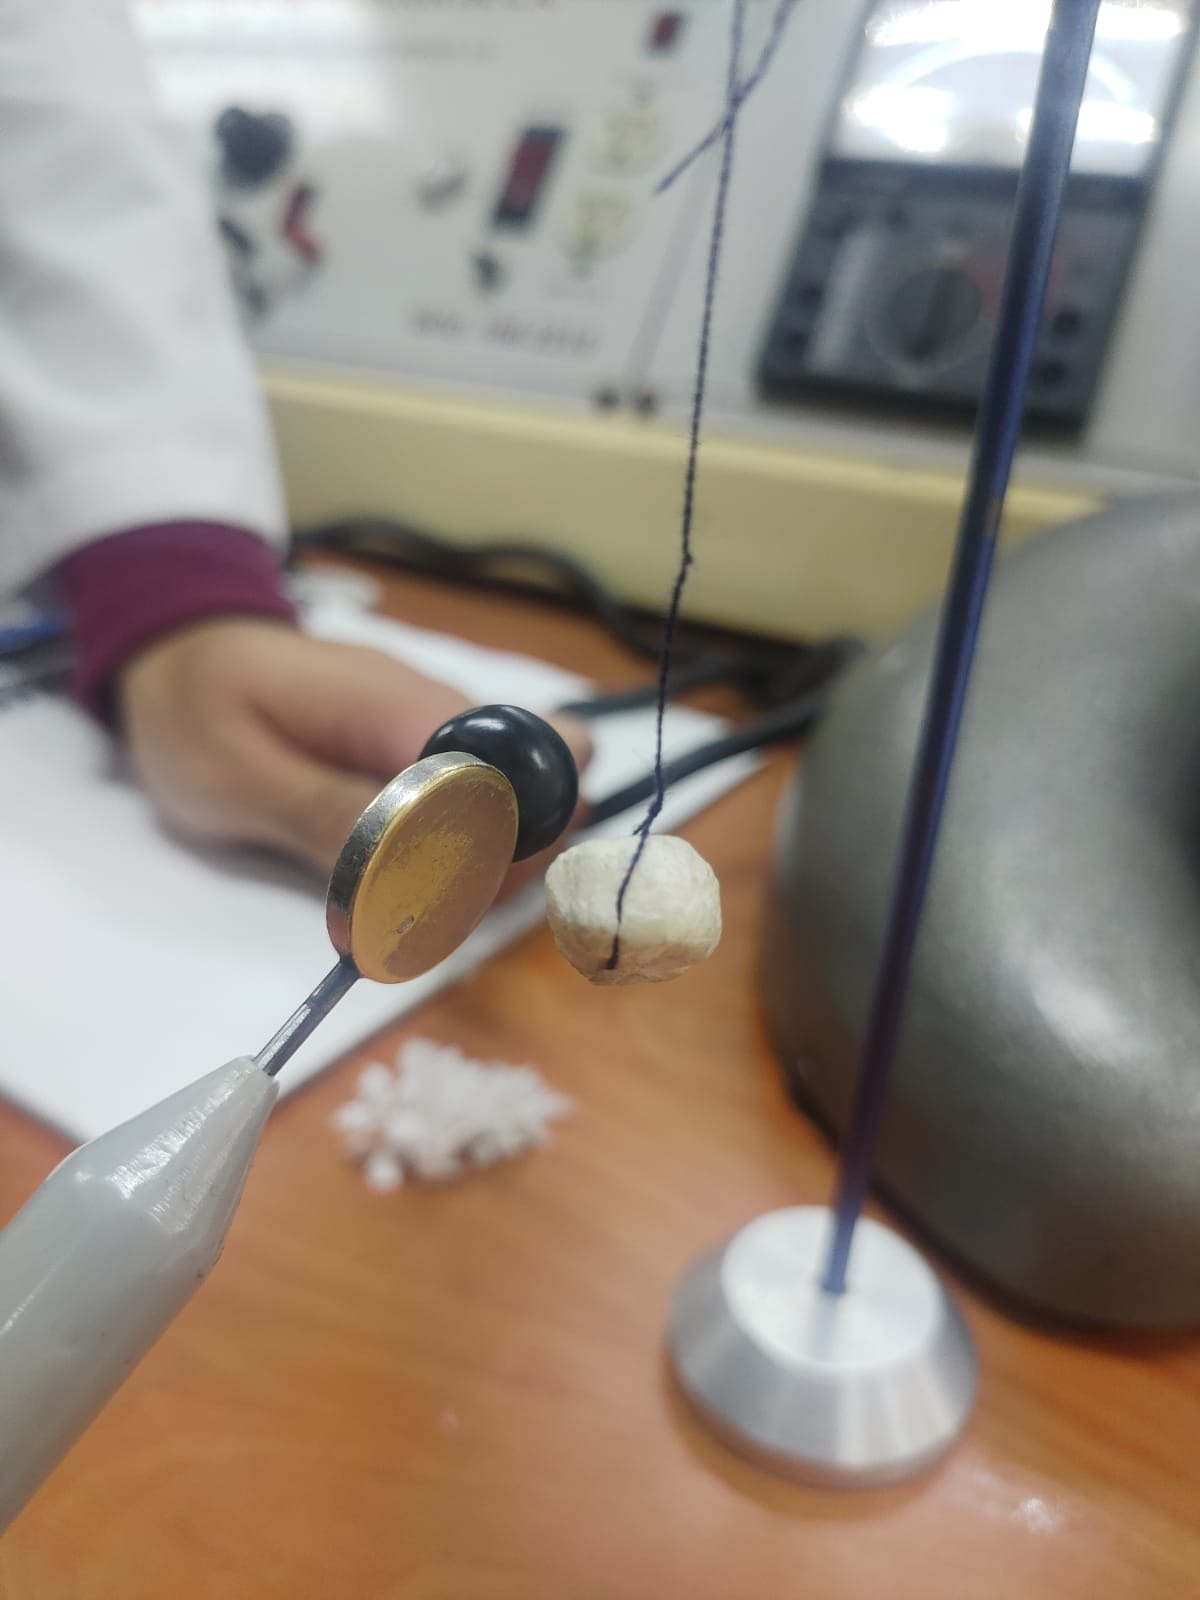
\includegraphics[scale=0.07]{P8}
\caption{Resultado}
\end{figure}

Como resultado observamos que al unir la barra de poliestireno y el electrodo de prueba plano, no genero ningún campo eléctrico, ya que la esfera de sauco  continuo en estado de reposo.                                                                    

\subsection*{1.3.- Electrización por inducción}
Para este experimento se va utilizar la barra de metal,y el pendulo electrico, y se tubo que armar de la siguiente manera:


\begin{figure}[h]
\centering
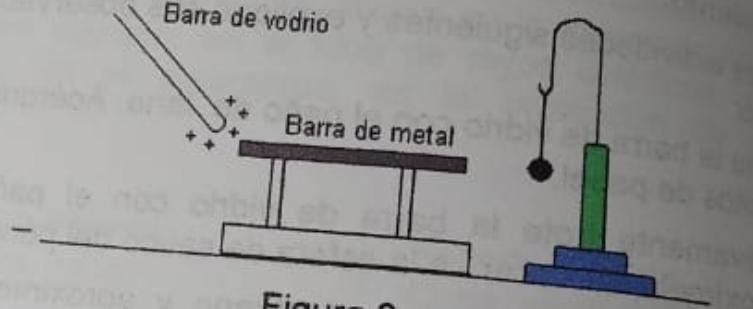
\includegraphics[scale=0.2]{P10}
\caption{Ejemplo}
\end{figure}

\subsubsection*{Procedimiento 1}
Se utilizo la barra de vidrio, cargada previamente por el frotamiento del paño de lana a si generando un campo eléctrico, acercamos la barra de vidrio a la barra de metal sin tocarla, luego observamos la esfera del péndulo eléctrico.

\begin{figure}[h]
\centering
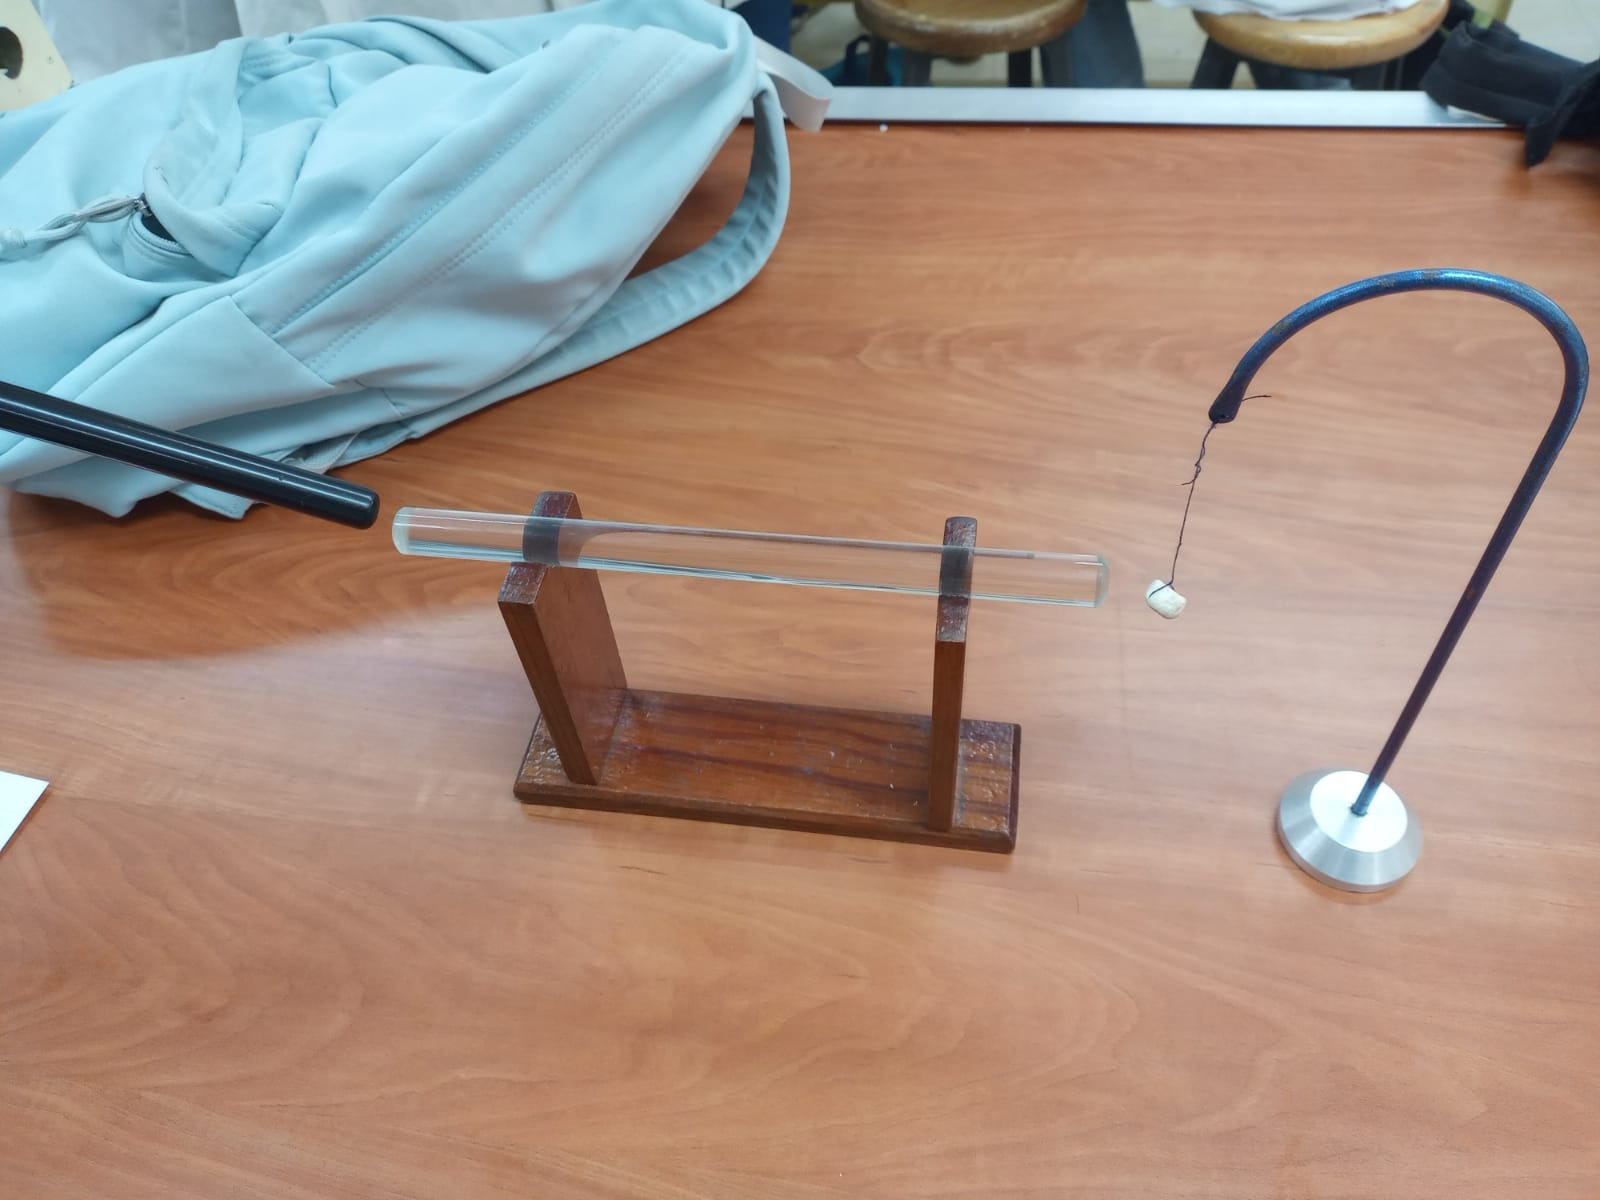
\includegraphics[scale=0.07]{P11}
\caption{Resultado}
\end{figure}

Como resultado observamos que al acercar la barra de vidrio con la barra de metal, genero una fuerza de atracción asi provocando que la esfera del péndulo eléctrico se moviera, tambien observamos que al porvocar el moviemto de la esfera del péndulo eléctrico, hizo que generara una pequeña chispa.
\subsection{Observaciones de los experimentos II y III}
Toque con la barra de vidrio, frotada con el paño de lana, la esfera de médula de sauco del péndulo durante un corto intervalo de tiempo. Anote sus observaciones. Descargue la esfera tocándola con los dedos y repita el procedimiento anterior empleando la barra de poliestireno. Anote sus observaciones. Explique lo ocurrido, obtenga sus conclusiones.
Podemos observar que al frotar la barra de vidrio con el paño de lana empieza a calentarse es decir empieza a tener una carga eléctrica, el vidrio adquiere carga positiva y el paño queda electrizada negativamente, acercamos la barra de vidrio a la esfera de medula del sauco del péndulo y esta empezó a descargarse en la esfera provocando que estas se acerquen y produzcan una carga eléctrica\\
\begin{figure}
	\begin{center}
		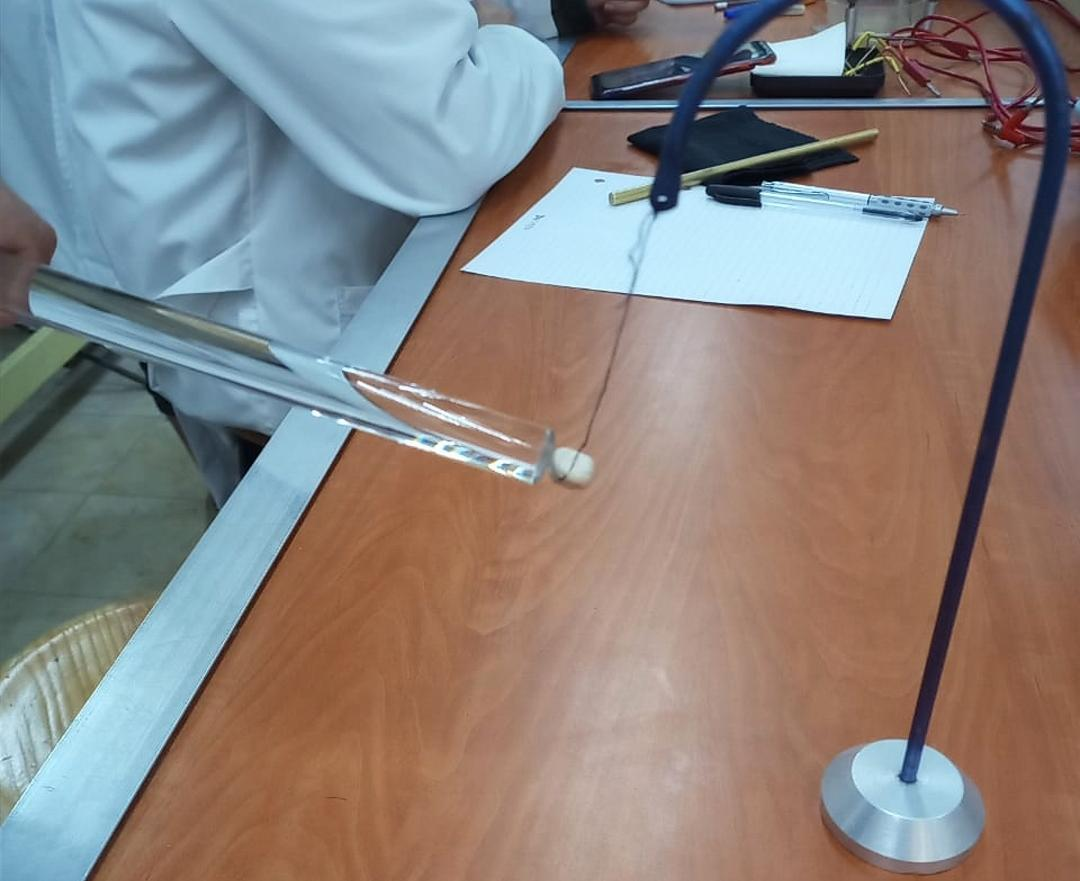
\includegraphics[width=0.2\textwidth]{Unos}\\

	\end{center}
\end{figure}

Descargamos la esfera tocándola con los dedos
Y repetimos el mismo procedimiento anterior empleando la barra de poliestireno. 
En este caso observamos lo mismo, la esfera de medula de sauco tiene carga negativa, mientras que la barra de poliestireno tiene carga positiva, por lo que se atraen entre sí.

La fuerza es mutua, la barra atrae a la esfera y la esfera atrae a la barra, pero es débil, incapaz de arrancar la barra de nuestra mano, cuando se electriza, la medula de sauco adquiere carga negativa, mientras que el poliestireno electrizado tiene carga positiva.\\
\begin{figure}
	\begin{center}
		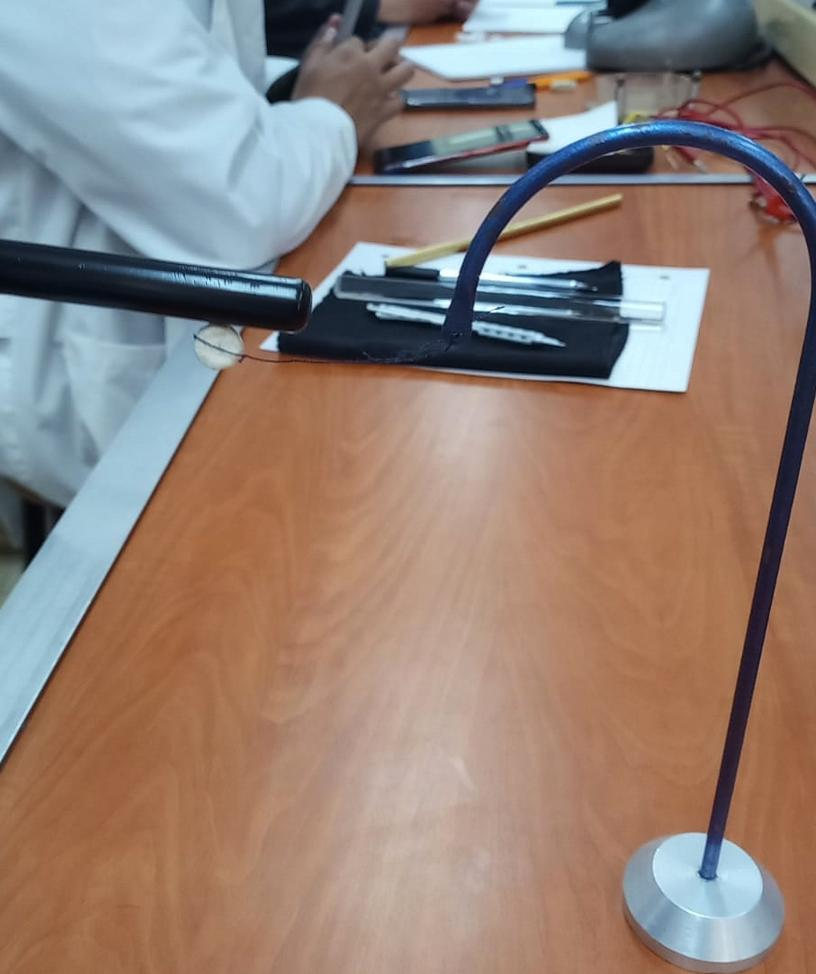
\includegraphics[width=0.2\textwidth]{Dos}\\

	\end{center}
\end{figure}

Después acercamos suficientemente la esfera cargada del péndulo eléctrico, sin hacer contacto, primero a la barra de vidrio cargada
Y después a la barra de poliestireno frotada con el paño de lana
 Explique sus observaciones y señale que sucede con el espacio que rodea a un cuerpo cargado.
A la barra de vidrio frotada con el paño queda con una carga eléctricamente positiva, mientras que la esfera tiene una carga negativa, tienden a atraerse y por ende la esfera se veía atraída hacia la barra de vidrio.
Mientras tanto que con la de poliestireno al frotar la barra con el trapo pasan algunos electrones del trapo a la barra. Por eso la barra queda cargada positivamente y la esfera tiene una carga negativa, estas de igual manera se atraen, pero sin tocarse ya que la fuerza que estamos ejerciendo no lo permite.

III. Procedimiento: Toque el extremo A de la barra de poliestireno con la barra de vidrio cargada, previamente, por frotamiento con el paño de lana. Observe el péndulo eléctrico. Descargue la barra de vidrio y colóquela en el soporte aislante, en lugar de la barra de poliestireno y cargue esta última repitiendo el experimento. Explique sus observaciones.
\begin{figure}[h]
	\center
	\subfloat{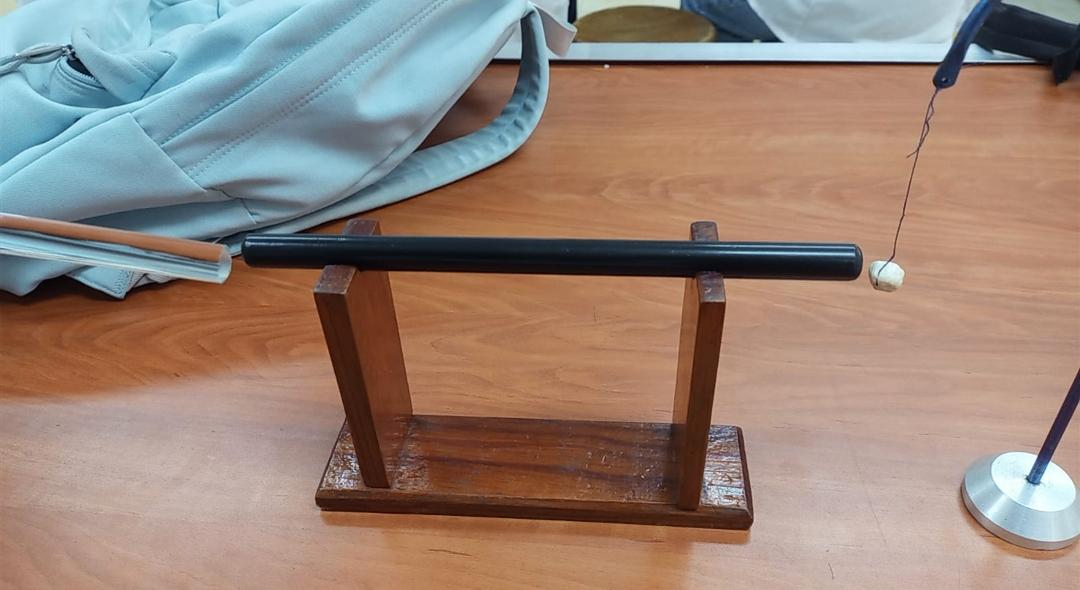
\includegraphics[width=0.2\textwidth]{Cuatros}}
	\hspace{0.3\textwidth}
	\subfloat{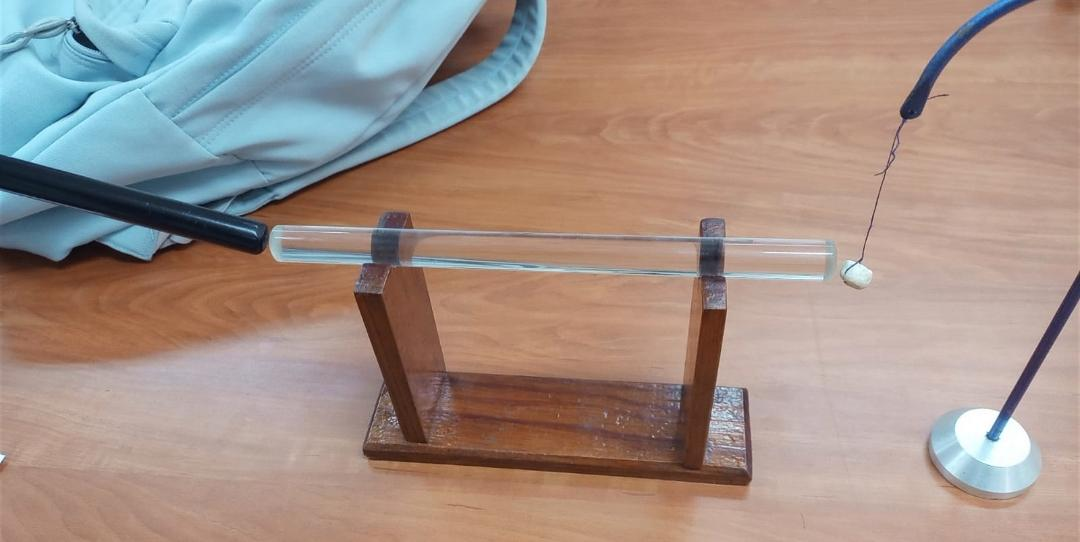
\includegraphics[width=0.2\textwidth]{Cincos}}
\end{figure}


Primero con la barra de vidrio cargada eléctricamente positiva, se acerca en el extremo de la barra de poliestireno este tiene carga neutra, mientras que la medula el sauco tiene una carga negativa, al cargar la barra de vidrio(+), transferimos esa carga a la barra de poliestireno provocando una atracción hacia la medula de sauco(-).

Repetimos el mismo procedimiento:
Se carga la barra de poliestireno eléctricamente positiva, lo acercamos en el extremo de la barra de vidrio ahora este tiene carga neutra, mientras que la medula el sauco tiene una carga negativa, al cargar la barra de poliestireno(+), transferimos esa carga a la barra de vidrio provocando una atracción hacia la medula de sauco(-).
\section{Experimento IV.}

Primeramente, antes de comenzar a realizar las observaciones del experimento, conozcamos la maquina que utilizamos para cargar nuestros electrodos, el generador de Van Graaff.

El funcionamiento es sencillo, un motor hace rodar una cinta sobre los rodillos que están hechos de material aislante que debido a la fricción acaban cargados, en el caso de la cinta, queda cargada negativamente por el interior y en el exterior de forma positiva.

En la parte superior e inferior existe un peine que reúne las cargas positivas, esto lo hace porque el rodillo superior queda cargado de forma positiva y repele a las cargas positivas en la cinta hacía el peine.Cuando la cinta regresa mantiene la carga negativa en su interior y esta carga es acumulada por el otro peine. Con esto podemos concluir que la polaridad es positiva en la superficie de la esfera metálica y negativa en la base del generador.

\begin{figure}[h!]
	\centering
	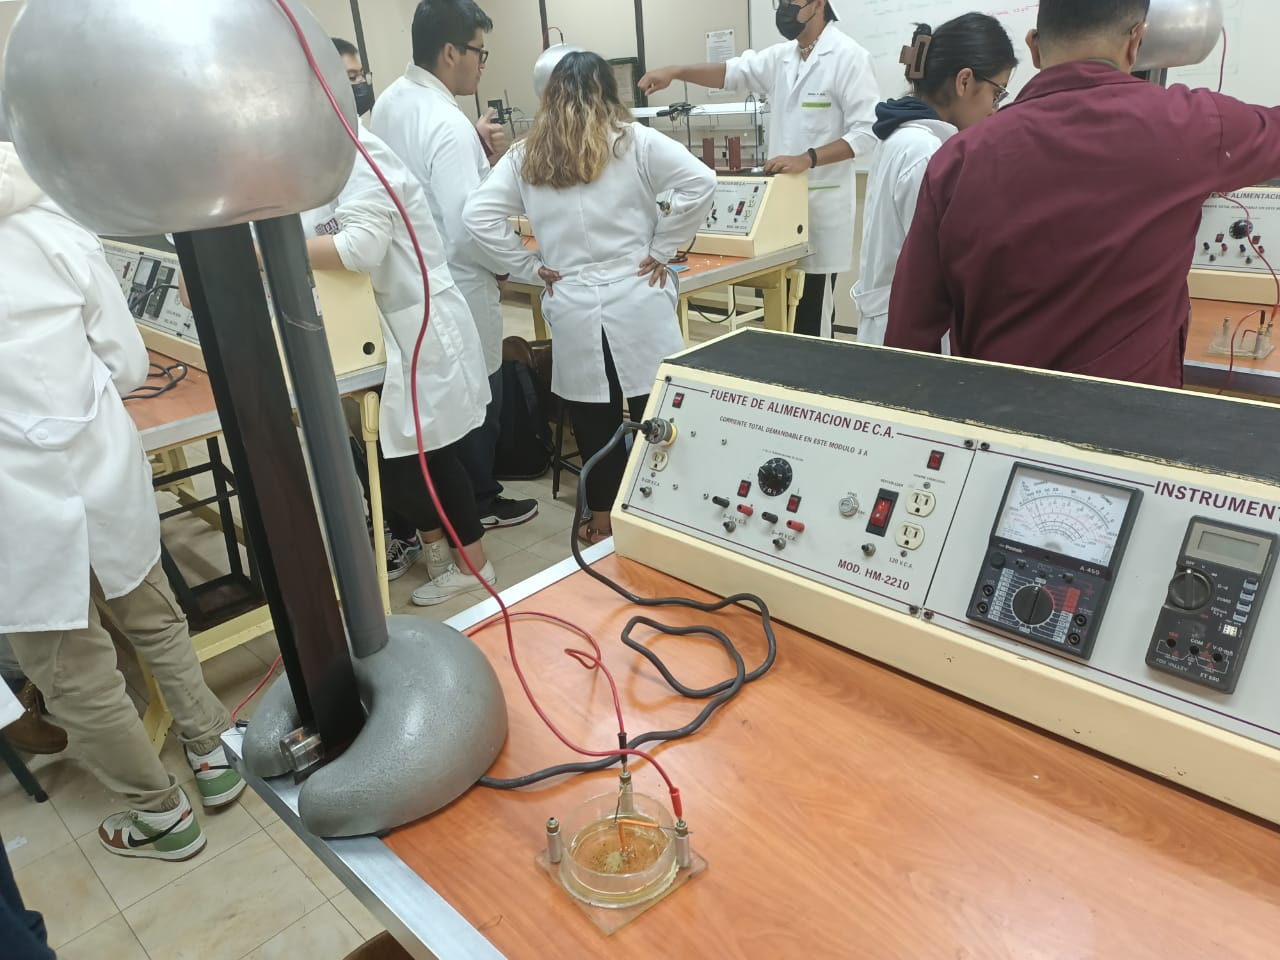
\includegraphics[scale=0.2]{Generador 2}
	\caption{Generador de Van Graaff}
	\label{fig:Generador}
	Observe que la punta roja es positiva y la punta negra negativa.
\end{figure}

Con esto aclarado, podemos comenzar a analizar los campos formados por la interacción de los pares de electrodos.


\subsection{Lenteja y arillo.}



La lenteja y el arillo poseen carga contraria.

\begin{figure}[h!]
	\centering
	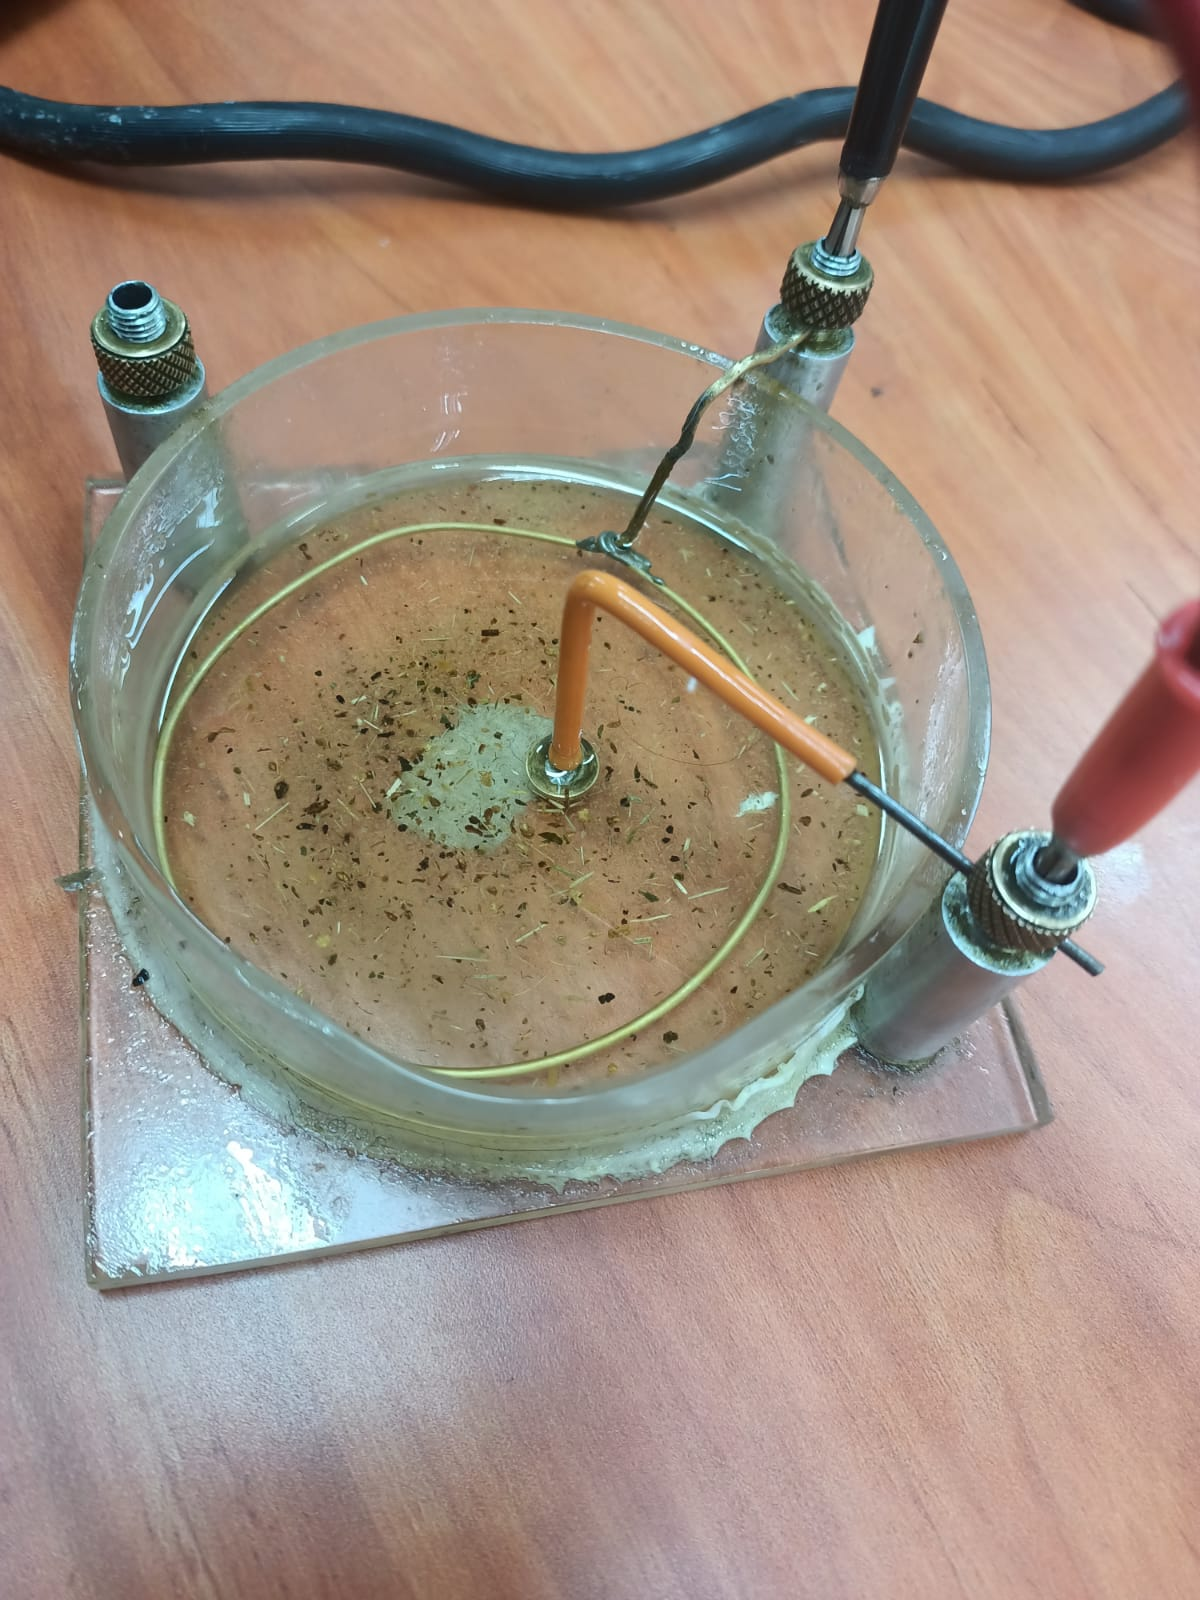
\includegraphics[scale=0.15]{Lenteja y anillo 1}
	\caption{Sistema con el generador apagado.}
	\label{fig:AyLO}
\end{figure}


\begin{figure}[h!]
	\centering
	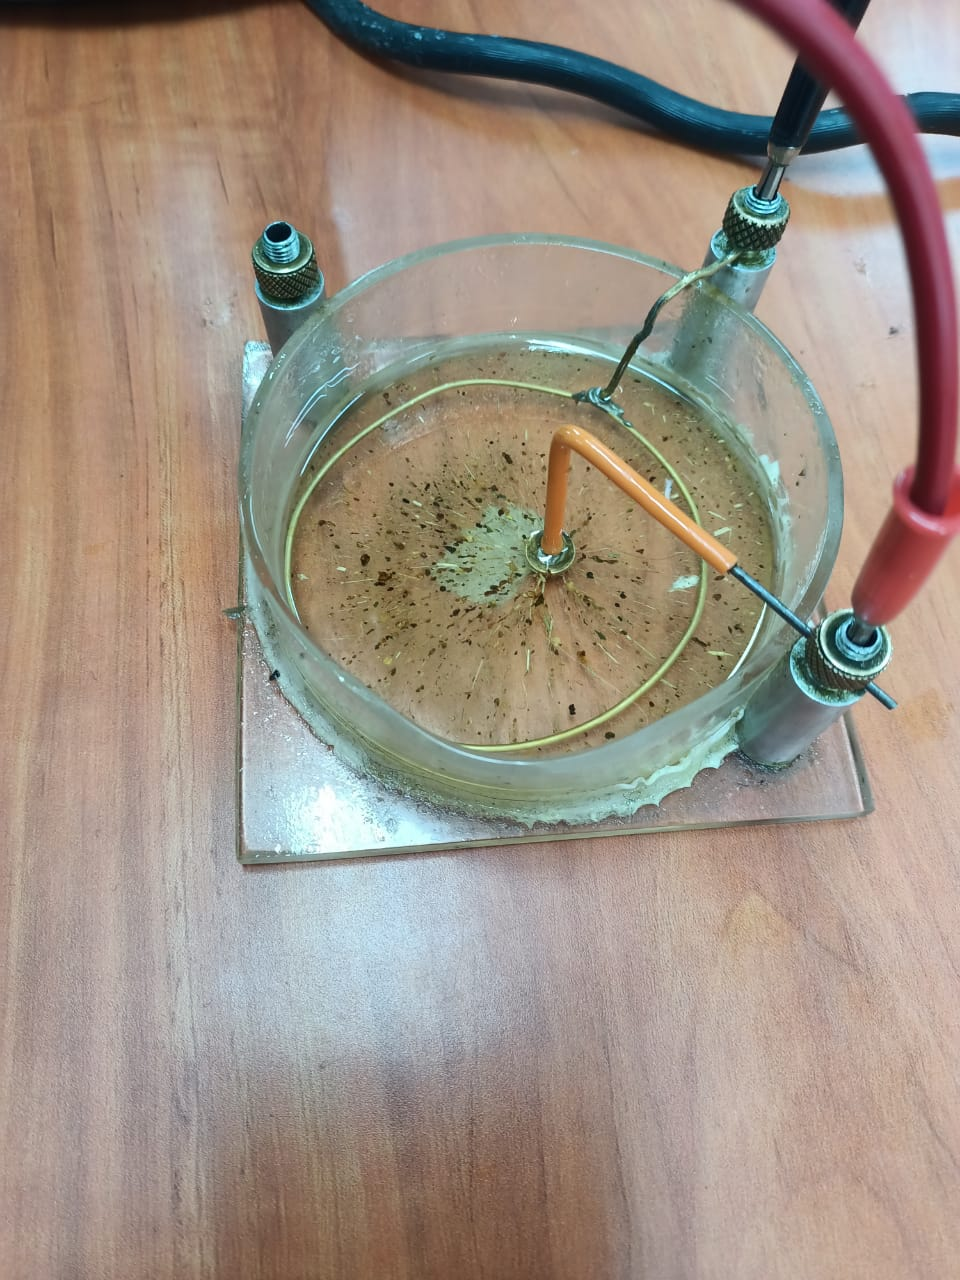
\includegraphics[scale=0.2]{Lenteja y anillo 2.1}
	\caption{Sistema con el generador encendido.}
	\label{fig:AyLE1}
\end{figure}

En la figura \ref{fig:AyLE1} se puede apreciar como el aserrín comienza a formar líneas al rededor de la lenteja y por fuera del anillo. Podemos notar también que según lo observado en la figura \ref{fig:Generador} el anillo posee una carga negativa y la lenteja positiva.


\begin{figure}[h!]
	\centering
	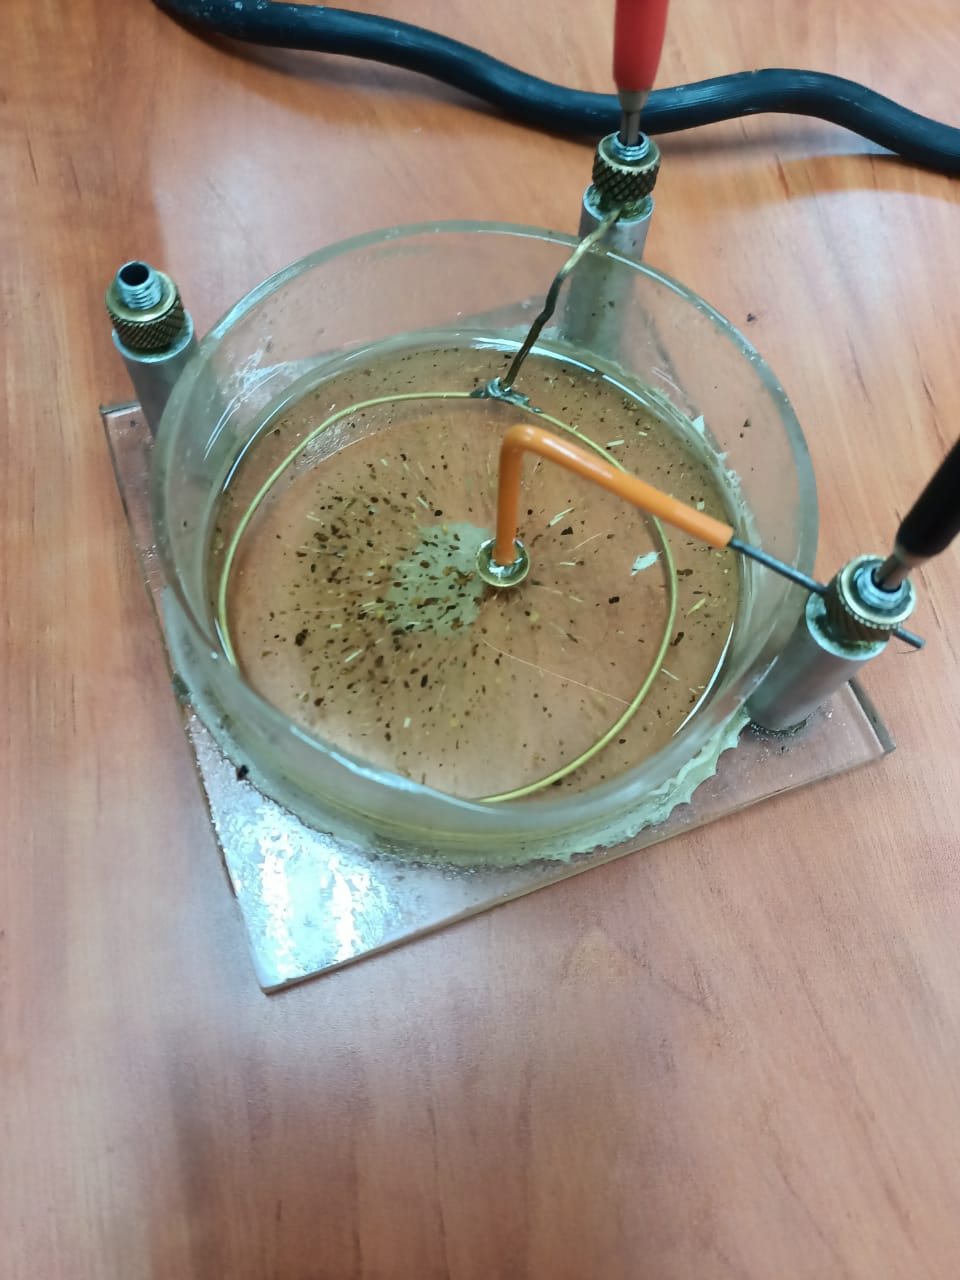
\includegraphics[scale=0.2]{Lenteja y anillo 2}
	\caption{Sistema con la polaridad invertida y el generador encendido.}
	\label{fig:AyLE2}
\end{figure}

En la figura \ref{fig:AyLE2} se aprecia nuevamente la formación de líneas al rededor de la lenteja y del anillo, en este caso, el anillo posee una carga positiva y la lenteja negativa. 

Dado a que es indistinguible la dirección del aserrín, se pueden hacer dibujos del campo eléctrico considerando la polaridad de las puntas ya establecida en la Figura \ref{fig:Generador}.

\begin{figure}[h!]
	\centering
	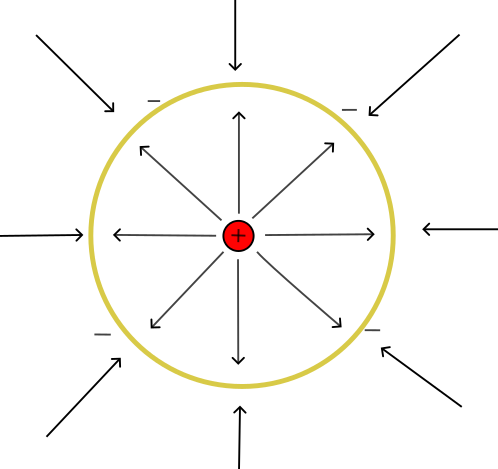
\includegraphics[scale=0.5]{a1}
	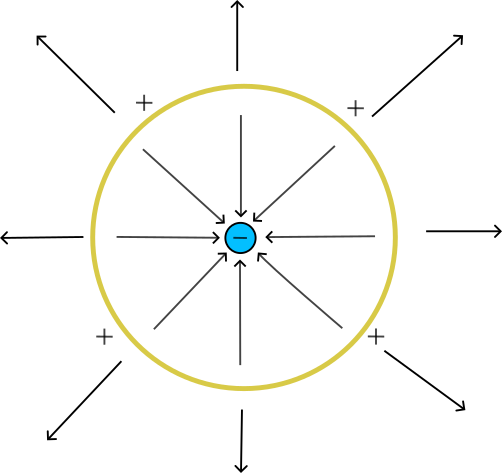
\includegraphics[scale=0.5]{a2}
	\caption{Líneas del campo eléctrico formado en la Figura \ref{fig:AyLE1} (izquierda) y la Figura \ref{fig:AyLE2} (derecha).}
\end{figure}


\subsection{Dos cargas puntuales de diferente signo.}

\begin{figure}[h!]
	\centering
	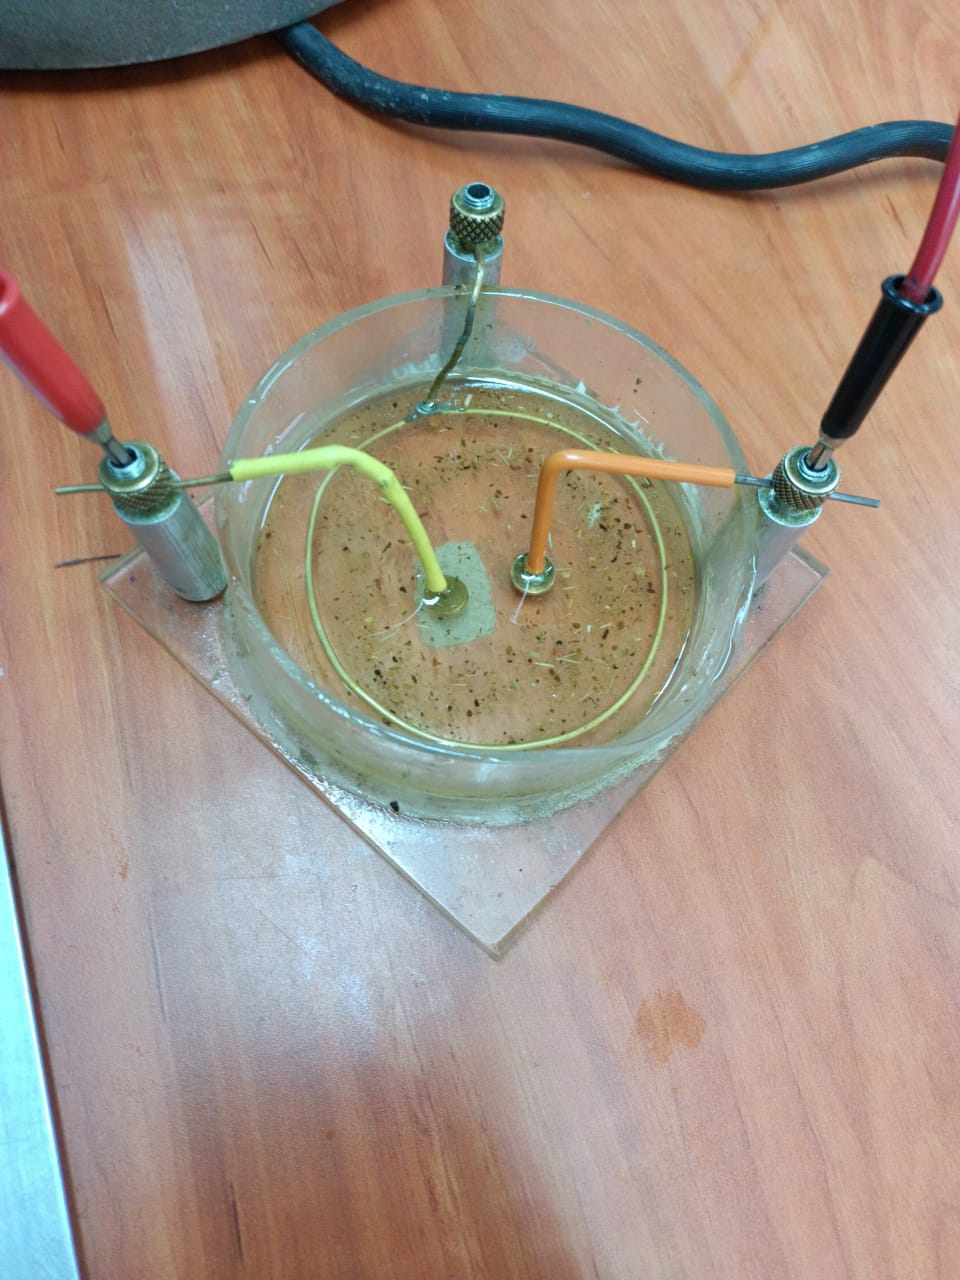
\includegraphics[scale=0.2]{Dos cargas Dif 1}
	\caption{Sistema con el generador apagado.}
\end{figure}

\begin{figure}[h!]
	\centering
	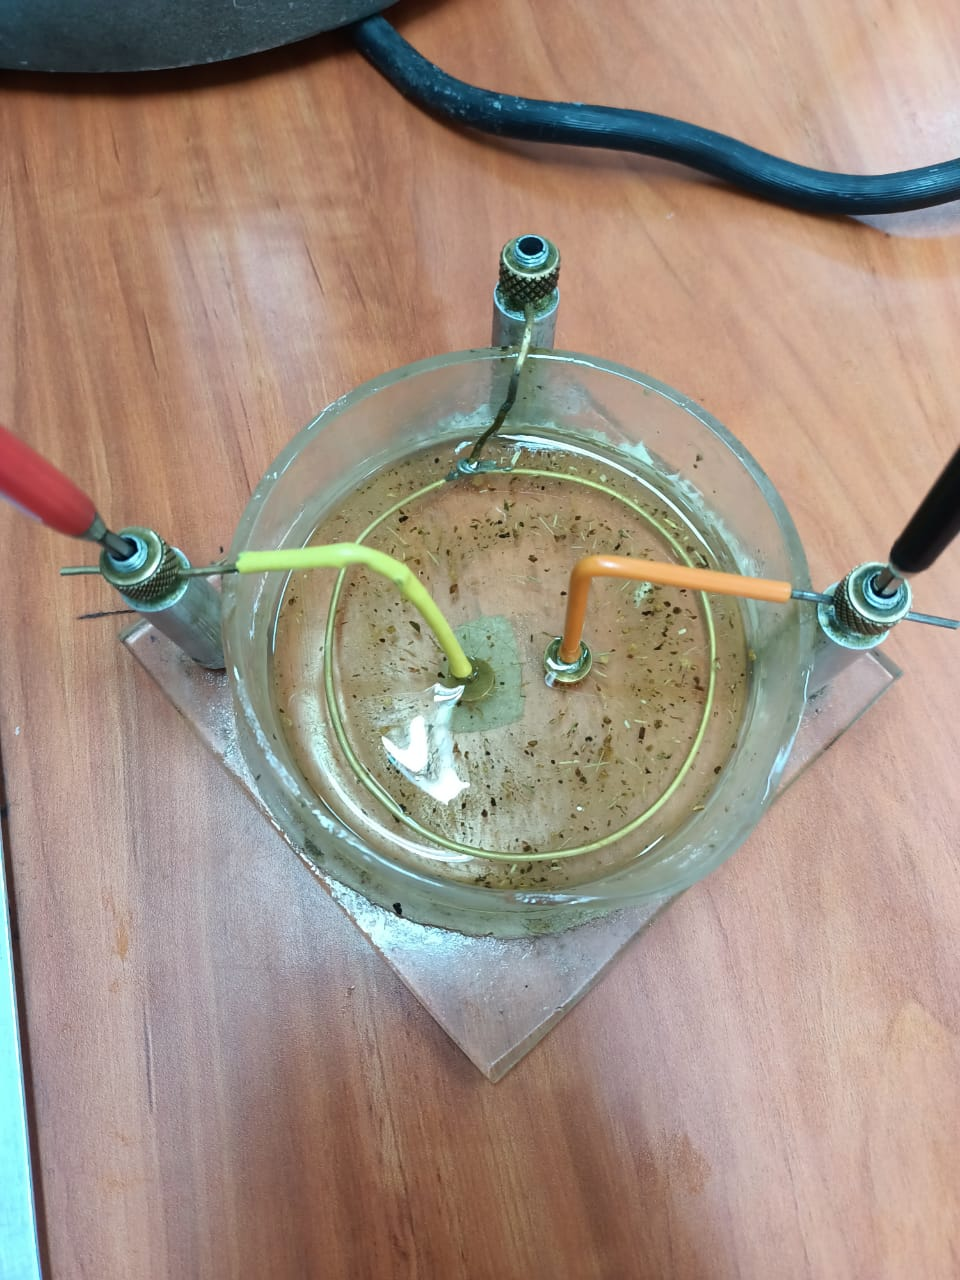
\includegraphics[scale=0.2]{Dos cargas Dif 2}
	\caption{Sistema con el generador encendido.}
	\label{fig:CDif1}
\end{figure}

En la Figura \ref{fig:CDif1} podemos observar ahora como el aserrín comienza a formar curvas. Nuevamente para describir mejor el comportamiento del campo eléctrico lo dibujaremos considerando la polaridad de los electrodos.

\begin{figure}[h!]
	\centering
	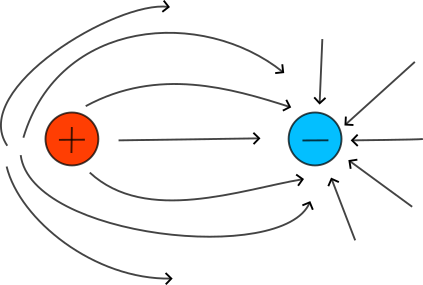
\includegraphics[scale=0.5]{b}
	\caption{Campo eléctrico formado en la Figura \ref{fig:CDif1}.}
	
\end{figure}


\subsection{Dos cargas puntuales del mismo signo.}

\begin{figure}[h!]
	\centering
	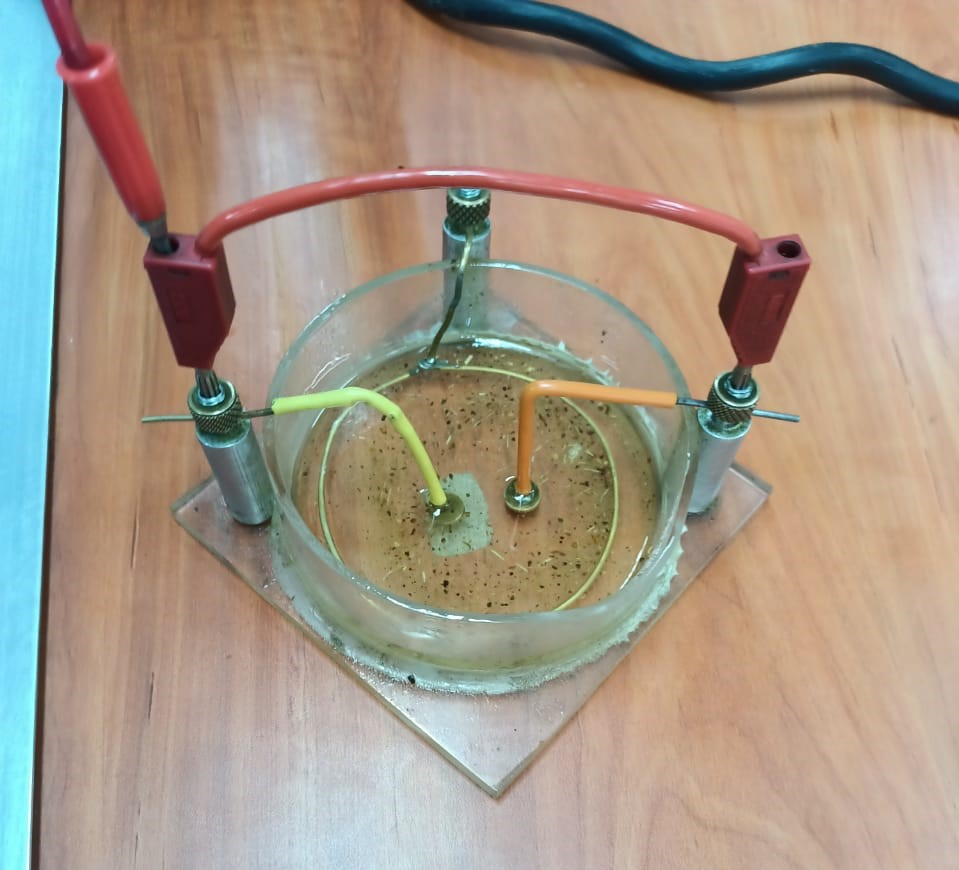
\includegraphics[scale=0.3]{Dos cargas Ig 1}
	\caption{Sistema con el generador apagado.}
	\label{fig:2CarIA}
\end{figure}

\begin{figure}[h!]
	\centering
	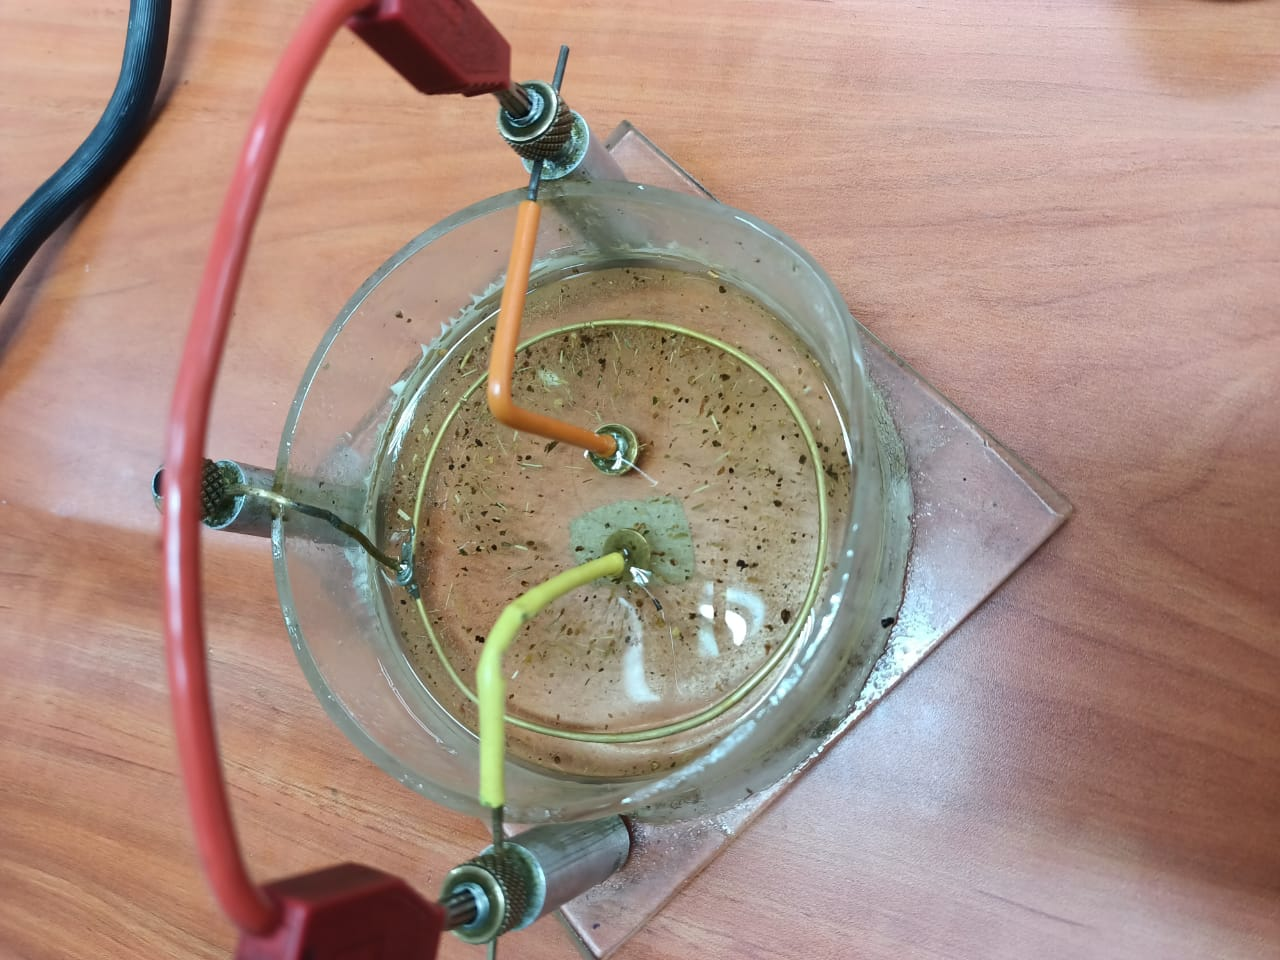
\includegraphics[scale=0.3]{Dos cargas Ig 2}
	\caption{Sistema con el generador encendido.}
	\label{fig:2CarI}
\end{figure}

En la Figura \ref{fig:2CarIA} podemos determinar que las dos cargas son positivas y en la Figura \ref{fig:2CarI} observamos nuevamente la formación de líneas pero con la particularidad que la parte media entre las dos cargas está vacía esto por la acción de la repulsión.

\begin{figure}
	\centering
	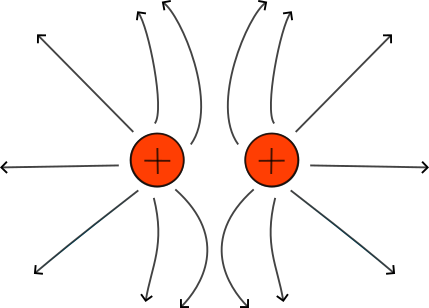
\includegraphics[scale=0.5]{c}
	\caption{Campo eléctrico formado en la Figura \ref{fig:2CarI}.}
\end{figure}

\subsection{Dos placas paralelas cargadas de diferente signo.}

\begin{figure}[h!]
	\centering
	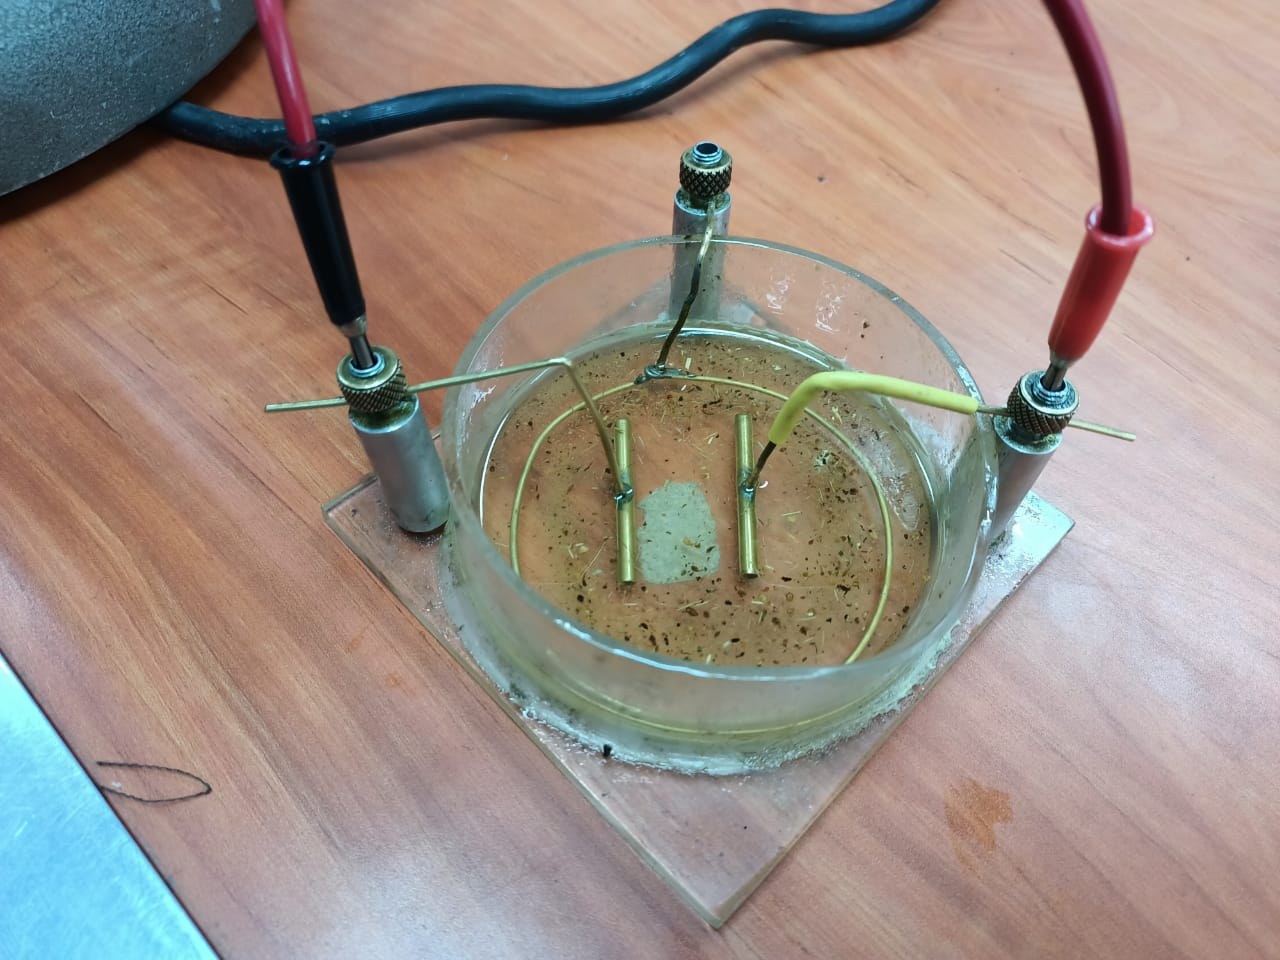
\includegraphics[scale=0.2]{Dos placas 1}
	\caption{Sistema con el generador apagado.}
\end{figure}

\begin{figure}[h!]
	\centering
	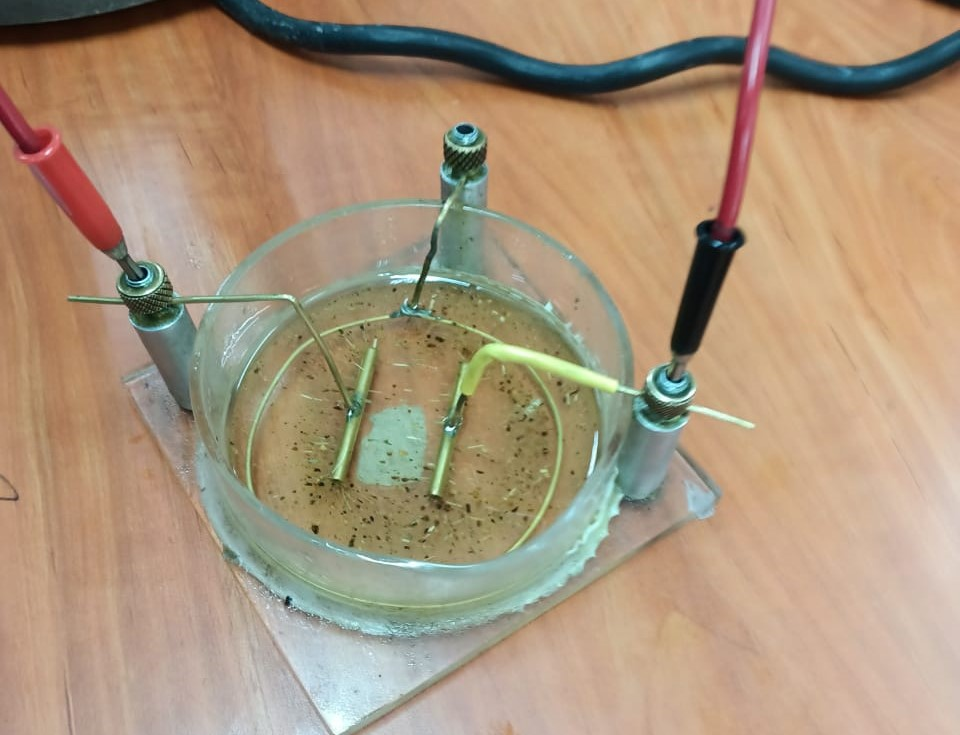
\includegraphics[scale=0.3]{Dos placas 2}
	\caption{Sistema con el generador encendido.}
	\label{fig:DosPlacas}
\end{figure}

En la figura \ref{fig:DosPlacas} podemos observar como entre las placas el aserrín forma la líneas paralelas y al rededor de los electrodos forman curvas.

\begin{figure}[h!]
	\centering
	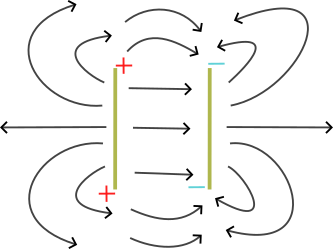
\includegraphics[scale=0.5]{d}
	\caption{Campo eléctrico formado en la Figura \ref{fig:DosPlacas}.}
\end{figure}


\subsection{Dos arillos circulares cargados con diferente carga}

\begin{figure}[h!]
	\centering
	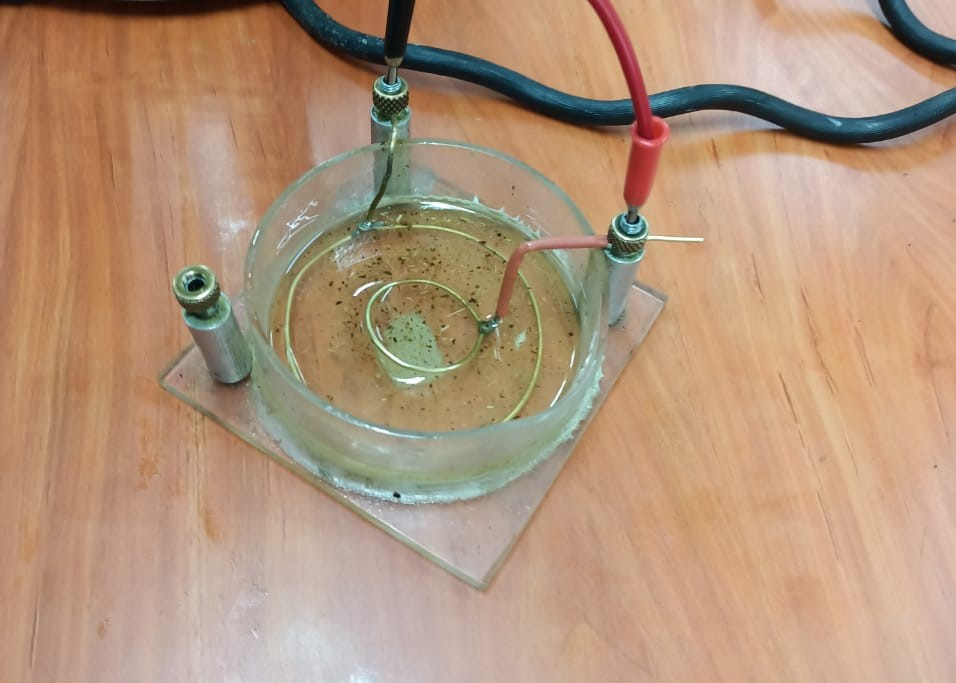
\includegraphics[scale=0.4]{Dos arillos 1}
	\caption{Sistema con el generador apagado.}
	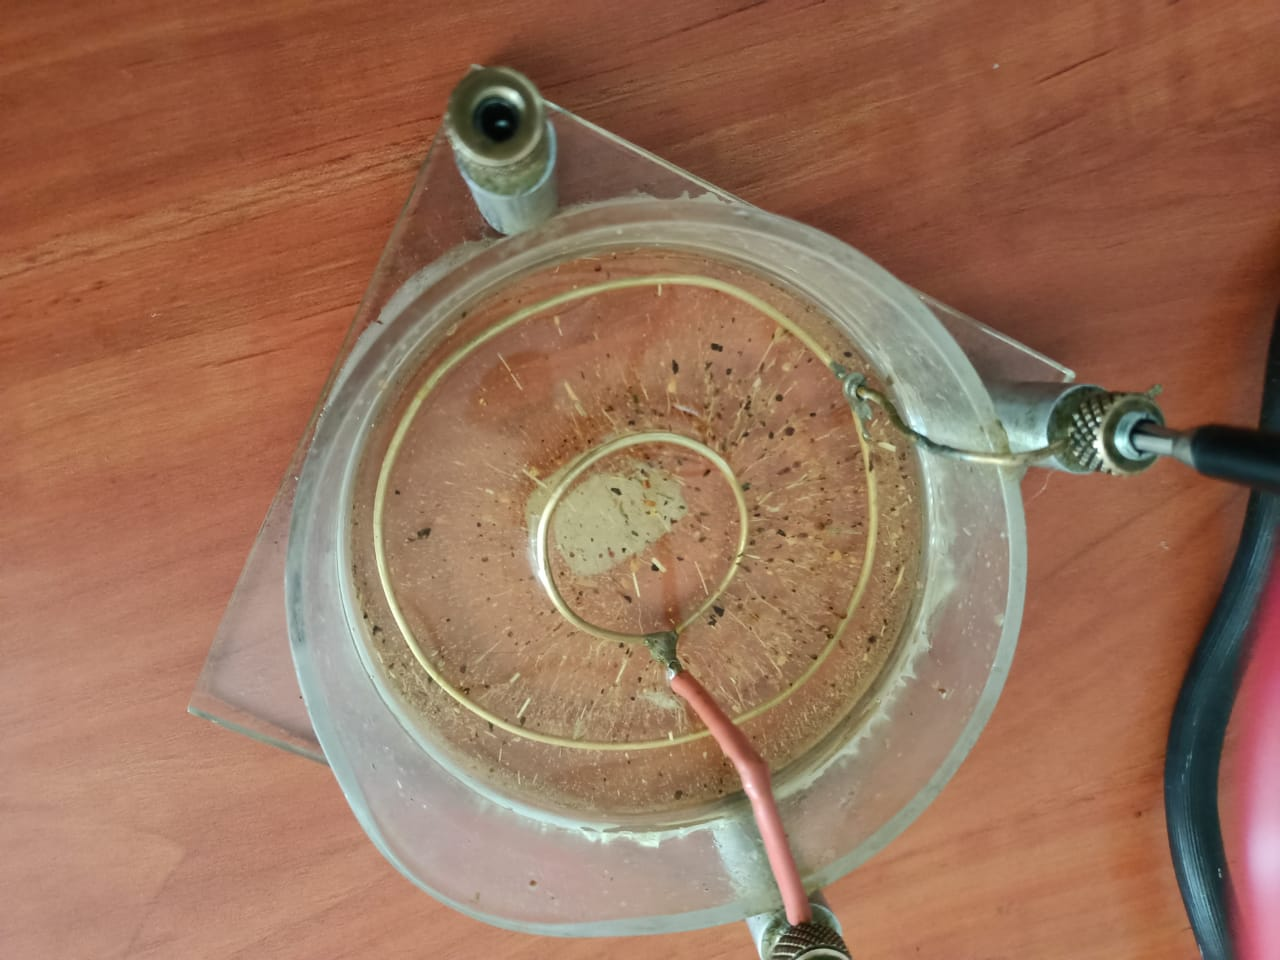
\includegraphics[scale=0.3]{Dos arillos 2}
	\caption{Sistema con el generador encendido.}
	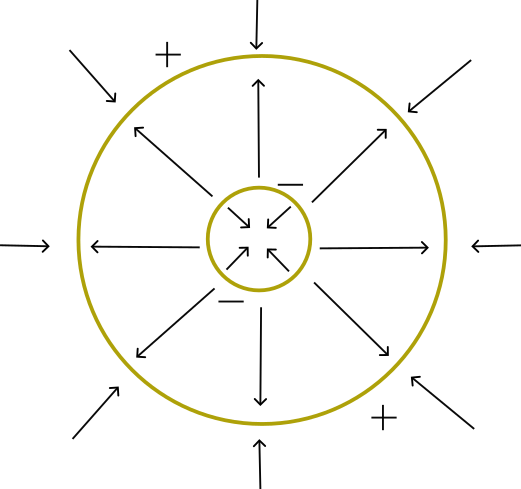
\includegraphics[scale=0.5]{e}
	\caption{Campo eléctrico formado en la figura 23}
\end{figure}

\clearpage
\newpage





\section{Conclusión}
\subsection{Grimaldi Díaz Uriel}

Durante la práctica pude observar las distintas formas electrificación de los cuerpos , la fricción , el contacto y la inducción , siendo de entre las 3 , la más presente , la fricción ya que con ella realizamos experimentos para observar la segunda y tercera, incluso nos apoyamos de una máquina que usa este efecto triboeléctrico (forma formal de llamar a la electrificación por frotamiento). Sin duda la parte más interesante de la práctica es el observar la acción de fuerzas invisibles para nuestros ojos pero que sin embargo tienen efecto en los cuerpos y por última instancia hacer estás fuerzas visibles por medio de la cubeta con ricino y aserrín y analizar la interacción de los campos eléctricos de los cuerpos según su naturaleza e incluso su forma geométrica. La importancia de lo aprendido en esta práctica radica en que es la base para entender procesos más complejos de generación eléctrica e incluso entender el concepto de magnetismo dado a que son fenómenos muy cercanos.
\subsection{Pérez Vargas Daniela Elizabeth}
La electrostática nos sirve para el estudio de los fenómenos eléctricos en reposo, es decir, las cargas eléctricas en equilibrio estático. Se basa en la Ley de Coulomb, en donde establece la fuerza de atracción o repulsión entre dos cargas eléctricas en función de magnitud y distancia. En esta practica hay un desequilibrio de cargas positivas y negativas entre los objetos, al frotar las barras con los paños de lana estas se cargan eléctricamente provocando que haya una atracción hacia la esfera. El campo eléctrico nos demuestra la influencia que una carga eléctrica ejerce sobre las cargas eléctricas que hay en su entorno, en nuestro caso sobre las barras, y la esfera.
\subsection{Jesus Martinez Amac}

Durante la práctica pudimos observar las formas de la electrostática, basadas por el frotamiento de distintos cuerpos, en base al frotamiento o fricción que realizamos con los distintos experimentos, basándonos con los instrumentos más importantes de la práctica llamados: péndulo eléctrico, generador de Van de Graaff. La parte más interesante para mí fue utilizar el generador de Van de Graaff con la cuba electrostática de aceite de ricino y aserrin, ya que pudimos observar las fuerzas que no son visibles a simple vista, así pudiendo observar que genera un campo eléctrico creado por la fuerza de atracción y repulsión de las cargas electricas.

\subsection{Hernández Huerta José Emilio}
En el mundo podemos experimentar diferente fenomenos electricos por nuestra propia cuenta, pero en este caso en especifico podemos experimentar en un ambiente controlado estos fenomenos, generando estatica con un motor especial. 
Podemos comprender que al generar una corriente electrica esta genera un campo electrico el cual atrae los fragmentos de aserrin estos campos se forman al rededor de los electrodos y dependiendo de su orientacion podemos ver y anticipar sus formaciones ya sean atrayendolas o repeliendolas. Comprendiendo de una mejor forma lo ya visto en las clases de teoria pero de una forma más grafica.

\subsection{Nataly Bejarano Garduño}
Observamos de una manera práctica la electrostática basada en los tipos de electrizacion, frotamiento, contacto y por inducción, siendo la de fricción la más constante.
Así mismo visualizar como se producen las cargas eléctricas en cada de los electrones, y como afectan en el campo eléctrico (ya que lo visualizamos con el aserrín).
Está última fue la parte más interesante de la práctica, ya que no es lo mismo la teoría, que la práctica, y de este modo pudimos observar mejor la reacción y entender mucho mejor el tema, ya que nos interesó más.

\clearpage
\newpage	
	\begin{thebibliography}{0}
		\bibitem{BC}Botero, A. F., Rueda, J. a. A., \& Granja, Á. D. G. (2020b). Electricidad y magnetismo: una guía introductoria.
		\bibitem{Electrostatica}Silvia Vettorel, Ignacio Tabares, \& Alicia Oliva. (n.d.). Electrostática 4° año (Primera). Universidad Nacional de Rosario.
		\bibitem{Sonora}[ Dr. Mario Enrique Álvarez Ramos, Dr. Roberto Pedro Duarte Zamorano, Dr. Ezequiel Rodríguez Jáuregui, \& Dr. Santos Jesús Castillo. (n.d.). Fisica II : Primera parte: Electricidad. Universidad de Sonora.
		\bibitem{Ñuñoa, Santiago.}Guía de estudio electrostática. (2019). New Heinrich High School.
	\end{thebibliography}
\end{document}